\documentclass[spanish]{extbook}
\usepackage[T1]{fontenc}
\usepackage[utf8]{inputenc}
%\usepackage[a4paper,showframe]{geometry}
\usepackage[a4paper]{geometry}
\usepackage{color}
\usepackage{amsmath}
\usepackage{graphicx}
\usepackage{listings}
\usepackage{float}
\usepackage[font=small,labelfont=bf]{caption}
\usepackage{graphicx}
\usepackage{parskip}
\usepackage[hidelinks]{hyperref}
\usepackage[capitalise]{cleveref}
\usepackage{bookmark}
\usepackage[spanish]{babel}
\usepackage{times}
\usepackage{color}

% for adjustwidth environment
\usepackage[strict]{changepage}

% for formal definitions
\usepackage{framed}

% environment derived from framed.sty: see leftbar environment definition
\definecolor{formalshade}{rgb}{0.95,0.95,1}
\definecolor{darkblue}{rgb}{0.0, 0.0, 0.55}

\newenvironment{tradnote}{%
  \def\FrameCommand{%
    \hspace{1pt}%
    {\color{darkblue}\vrule width 2pt}%
    {\color{formalshade}\vrule width 4pt}%
    \colorbox{formalshade}%
  }%
  \vspace{12pt}
  \MakeFramed{\advance\hsize-\width\FrameRestore}%
  \noindent\hspace{-4.55pt}% disable indenting first paragraph
  \begin{adjustwidth}{}{7pt}%
  \vspace{1pt}%
  \textbf{Nota del Traductor:\\}%
}
{%
  \vspace{6pt}\end{adjustwidth}\endMakeFramed%
}


\definecolor{gray97}{gray}{.97}
\definecolor{gray75}{gray}{.75}
\definecolor{gray45}{gray}{.45}

\crefdefaultlabelformat{\textbf{#2#1#3}}
\crefname{figure}{\textbf{Fig.}}{\textbf{Figures}}

\geometry{verbose}
\makeatletter
\numberwithin{equation}{section}
\numberwithin{figure}{section}
\makeatother
\addto\shorthandsspanish{\spanishdeactivate{~<>}}
\renewcommand{\lstlistingname}{Listado de código}
\setlength{\parindent}{0pt}
\renewcommand{\baselinestretch}{0.96}

\usepackage{listings}
\usepackage{color}

\lstset{ frame=Ltb,
     framerule=0pt,
     aboveskip=0.5cm,
     framextopmargin=3pt,
     framexbottommargin=3pt,
     framexleftmargin=0.4cm,
     framesep=0pt,
     rulesep=.4pt,
     backgroundcolor=\color{gray97},
     rulesepcolor=\color{black},
     %
     stringstyle=\ttfamily,
     showstringspaces = false,
     basicstyle=\small\ttfamily,
     commentstyle=\color{gray45},
     keywordstyle=\bfseries,
     %
     numbers=left,
     numbersep=15pt,
     numberstyle=\tiny,
     numberfirstline = false,
     breaklines=true,
   }
 
% minimizar fragmentado de listados
\lstnewenvironment{listing}[1][]
   {\lstset{#1}\pagebreak[0]}{\pagebreak[0]}
 
\lstdefinestyle{consola}
   {basicstyle=\scriptsize\bf\ttfamily,
    backgroundcolor=\color{gray75},
   }
 
\lstdefinestyle{R}
{
	language=R,
}

\definecolor{dkgreen}{rgb}{0,0.6,0}
\definecolor{gray}{rgb}{0.5,0.5,0.5}
\definecolor{mauve}{rgb}{0.58,0,0.82}

%%%%%%%%%%%%%%%%%%%%%%%%%%%%%%%%%%%%%%%%%%%%%%%%%%%%%%%%%%%%%%%%%%%%%%%%%%%%%%%
% Estilo del código
%%%%%%%%%%%%%%%%%%%%%%%%%%%%%%%%%%%%%%%%%%%%%%%%%%%%%%%%%%%%%%%%%%%%%%%%%%%%%%%
\lstset{frame=tb,
  language=R,
  aboveskip=3mm,
  belowskip=3mm,
  showstringspaces=false,
  columns=flexible,
  basicstyle={\small\ttfamily},
  numbers=none,
  numberstyle=\tiny\color{gray},
  keywordstyle=\color{blue},
  commentstyle=\color{dkgreen},
  stringstyle=\color{mauve},
  breaklines=true,
  breakatwhitespace=true,
  tabsize=3
}

\title{Introducción a las estadísticas con R}
\date{2018-01-20}
\author{Peter Daalgard\\\small{Traducido al español por Patricio Moracho}}
\begin{document}
\maketitle

%%%%%%%%%%%%%%%%%%%%%%%%%%%%%%%%%%%%%%%%%%%%%%%%%%%%%%%%%%%%%%%%%%%%%%%%%%%%%%%
%% Prefacio
%%%%%%%%%%%%%%%%%%%%%%%%%%%%%%%%%%%%%%%%%%%%%%%%%%%%%%%%%%%%%%%%%%%%%%%%%%%%%%%
\chapter*{Prefacio}

\textbf{R} es un programa informático para estadístas, disponible a través de
Internet bajo la Licencia Pública General (\textbf{GPL}). Es decir, se
suministra con una licencia que nos permite utilizarlo libremente, distribuirlo
o incluso venderlo, siempre que el receptor tenga los mismos derechos y el
código fuente esté disponible libremente. Existen versiones para Microsoft
Windows XP o posteriores, para una variedad de plataformas Unix y Linux, y para
Apple Macintosh OS X. 

\textbf{R} proporciona un entorno en el que puede realizar análisis
estadísticos y producir gráficos.  En realidad es un lenguaje de programación
completo, aunque eso, en este libro sólo se describe marginalmente. Aquí nos
conformamos con aprender los conceptos elementales y ver varios ejemplos. 

\textbf{R} está diseñado de tal manera que siempre es posible realizar más
cálculos sobre los resultados de un procedimiento estadístico. Además, la
funcionalidad para la presentación gráfica de los datos permite tanto métodos
simples, como por ejemplo \texttt{plot(x, y)}, como también la posibilidad de
un control mucho más fino del aspecto de las gráficas. 

El hecho que \textbf{R} esté basado en un lenguaje formal de computadora le da
una tremenda flexibilidad.  Otros sistemas presentan interfaces más sencillas
en términos de menús y formularios, pero a menudo la aparente facilidad de uso
se convierte en un obstáculo a largo plazo. Aunque las estadísticas elementales
se presentan a menudo como una colección de procedimientos fijos, el análisis
de datos moderadamente complejos requiere la creación de modelos estadísticos
ad-hoc, lo que hace que la flexibilidad añadida de \textbf{R} sea altamente
deseable.

\textbf{R} debe su nombre a una típica humorada de Internet. Es posible que
haya oído hablar del lenguaje de programación C (cuyo nombre es otra historia
en sí misma). Inspirados por esto, Becker y Chambers eligieron, a principios de
los años ochenta, llamar a su nuevo lenguaje de programación estadística S.
Este lenguaje se desarrolló aún más con el producto comercial S-PLUS, que a
finales de la década era de uso generalizado entre los estadísticos de todo
tipo. Ross Ihaka y Robert Gentleman de la Universidad de Auckland, Nueva
Zelanda, eligieron escribir una versión reducida de S para propósitos de
enseñanza, y ¿qué era más natural que elegir la letra inmediatamente anterior?
Las iniciales de Ross y Robert también pueden haber jugado un papel importante
en la elección del nombre.

En 1995, Martin Maechler persuadió a Ross y Robert para que publicaran el
código fuente de \textbf{R} bajo la licencia \textbf{GPL}. Esto coincidió con
el auge del software de código abierto impulsado por el sistema Linux.
\textbf{R} pronto logró llenar un hueco en gente como yo que tenía la intención
de usar Linux para computación estadística, pero no tenía ningún paquete
estadístico disponible en ese momento. Se creó una lista de correo para la
comunicación de informes de fallos y discusiones sobre el desarrollo de
\textbf{R}.

En agosto de 1997, me invitaron a unirme a un equipo internacional extendido
cuyos miembros colaboran a través de Internet y que ha controlado el desarrollo
de \textbf{R} desde entonces. Posteriormente, el equipo básico se amplió varias
veces y actualmente cuenta con 19 miembros. El 29 de febrero de 2000, se
publicó la versión 1.0.0.0. Al momento de este escrito, la versión actual es la
2.6.2. Este libro se basó originalmente en una serie de notas elaboradas para
el curso de Estadística Básica para Investigadores en Salud de la Facultad de
Ciencias de la Salud de la Universidad de Copenhague. El curso tenía como
objetivo principal, los estudiantes del doctorado en medicina. Sin embargo, el
material se ha revisado sustancialmente y espero que sea útil para un público
más amplio, aunque sigue habiendo algunos sesgos bioestadísticos, especialmente
en la elección de ejemplos. En los últimos años, el curso de Práctica
Estadística en Epidemiología, que se ha celebrado anualmente en Tartu
(Estonia), ha sido una fuente importante de inspiración y experiencia en la
introducción de jóvenes estadísticos y epidemiólogos a \textbf{R}.  Este libro
no es un manual para \textbf{R}.  La idea es introducir una serie de conceptos
y técnicas básicas que deberían permitir al lector comenzar con estadísticas
prácticas. En cuanto a los métodos prácticos, el libro cubre una currícula
razonable para los estudiantes de primer año de estadística teórica, así como
para los estudiantes de ingeniería. Estos grupos eventualmente necesitarán ir
más allá y estudiar modelos más complejos, así como técnicas generales que
involucren programación real en el lenguaje \textbf{R}.

Para los áreas en las que las estadísticas elementales se enseñan
principalmente como una herramienta, el libro va un poco más allá de lo que se
enseña comúnmente a nivel universitario. Los métodos de regresión múltiple o el
análisis de experimentos multifactoriales rara vez se enseñan a ese nivel, pero
pueden convertirse rápidamente en esenciales para la investigación práctica. He
recopilado los métodos más simples al principio para hacer el libro más legible
también en un nivel elemental. Sin embargo, para mantener el material técnico
consistente, los capítulos 1 y 2 sí incluyen material que algunos lectores
querrán omitir. Por lo tanto, el libro pretende ser útil para varios grupos,
pero no pretenderé que pueda valerse por sí solo para ninguno de ellos. He
incluido breves secciones teóricas en relación con los diversos métodos, pero
más que como material didáctico, éstos deberían servir de recordatorios o
quizás como aperitivos para los lectores que son nuevos en el mundo de la
estadística.



\cleardoublepage
\pdfbookmark{\contentsname}{Contenido}
\tableofcontents

%%%%%%%%%%%%%%%%%%%%%%%%%%%%%%%%%%%%%%%%%%%%%%%%%%%%%%%%%%%%%%%%%%%%%%%%%%%%%%%
%% Conceptos Básicos
%%%%%%%%%%%%%%%%%%%%%%%%%%%%%%%%%%%%%%%%%%%%%%%%%%%%%%%%%%%%%%%%%%%%%%%%%%%%%%%
\chapter{Conceptos Básicos}

El propósito de este capítulo es que empiece a usar  \textbf{R}.  Asumimos que
ya tiene una instalación funcional del software y del paquete \texttt{ISwR} que
contiene los conjuntos de datos para este libro. Las instrucciones para obtener
e instalar el software se encuentran en el \index{Apéndice A}. Como ya
mencionamos, el libro describe la versión 2.6.2 de  \textbf{R}.  En la medida
de lo posible, presento los temas de una manera que es independiente del
sistema operativo en uso y asumo que el lector tiene el conocimiento operativo
elemental para seleccionar desde menús, mover ventanas, etc. Sin embargo, hago
excepciones cuando soy consciente de dificultades específicas con una
plataforma o características específicas de la misma.

\begin{tradnote} 
	Al momento de la traducción la versión actual de R es la
	3.4.2, aún así, lo ejemplos y el código en general del libro son totalmente
	consistentes con las nuevas versiones. Asimismo es importante notar que el
	autor se centra en la forma estándar y básica de introducir comandos,
	directamente trabajando sobre la consola \textbf{R}, sin embargo, el lector
	puede trabajar con entornos más complejos de desarrollo como
	\textbf{Rstudio} que no debería significar grandes diferencias.
\end{tradnote} \newpage

%%%%%%%%%%%%%%%%%%%%%%%%%%%%%%%%%%%%%%%%%%%%%%%%%%%%%%%%%%%%%%%%%%%%%%%%%%%%%%%
%% Primeros pasos
%%%%%%%%%%%%%%%%%%%%%%%%%%%%%%%%%%%%%%%%%%%%%%%%%%%%%%%%%%%%%%%%%%%%%%%%%%%%%%%
\section{Primeros pasos}

Esta sección ofrece una introducción al entorno informático de  \textbf{R}
Computing y le muestra sus características más básicas. Iniciar  \textbf{R} es
sencillo, pero el método dependerá de su plataforma informática.  Podrá
iniciarlo desde el menú del sistema, haciendo doble clic en un icono o
introduciendo el comando \textquotedbl{}R\textquotedbl{} en la línea de
comandos del sistema. Esto producirá una ventana de consola o hará que
\textbf{R} se inicie como un programa interactivo en la ventana del terminal
actual. 

\begin{figure}[H]
  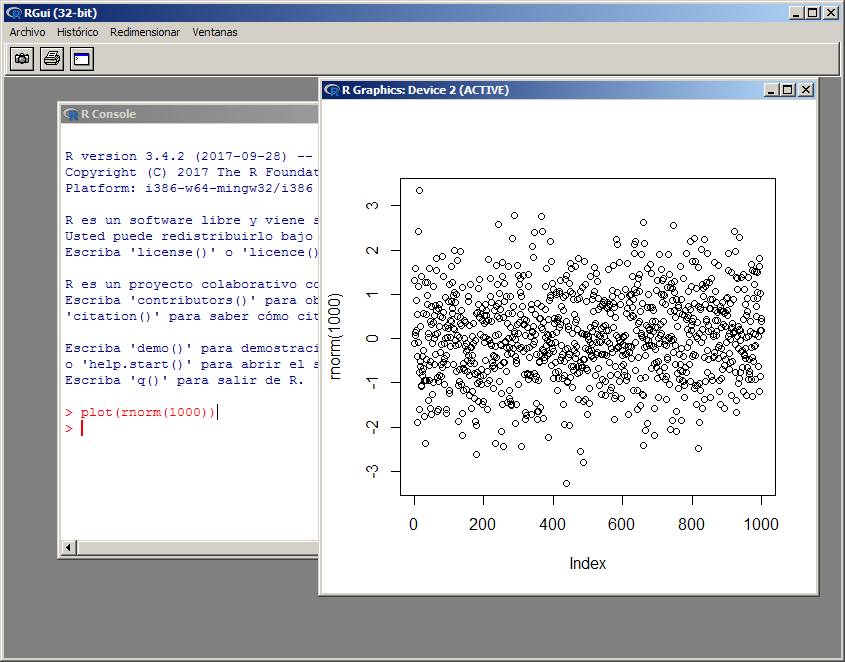
\includegraphics[width=\linewidth]{fig-1.png}
  \caption{Captura de patalla de R Windows.}
  \label{fig:fig-1}
\end{figure}

En cualquier caso, R funciona fundamentalmente según el modelo de
preguntas y respuestas:

Ingrese una línea con un comando y pulse \texttt{<ENTER>} (\texttt{<--}).
Entonces el programa hace algo, imprime el resultado si es relevante y pide más
información.

Cuando \textbf{R} está listo para la entrada, imprime su símbolo, un
\textquotedbl{}>\textquotedbl{}.  Es posible usar \textbf{R} como una
aplicación en modo sólo texto, y también en el modo por lotes, pero para los
propósitos de este capítulo, asumo que usted está sentado en una estación de
trabajo gráfica.

Todos los ejemplos de este libro deberían ejecutarse si los escribes
exactamente como están impresos, siempre y cuando tengas el paquete
\texttt{ISwR} no sólo instalado sino también cargado en tu ruta de búsqueda
actual. Esto se hace introduciendo:
\newpage

\begin{lstlisting}[language=R]
> library(ISwR)
\end{lstlisting}

en la línea de comandos. No necesita entender lo que hace este comando en este
preciso momento. Se explicará en la Sección 2.1.5. Para una primera impresión de
lo que \textbf{R} puede hacer, intente escribir lo siguiente:

\begin{lstlisting}[language=R]
> plot(rnorm(1000))
\end{lstlisting}

Este comando dibuja 1000 números al azar a partir de la distribución normal
(rnorm = \emph{r}andom \emph{norm}al) y los dibuja en una ventana emergente de
gráficos. El resultado en una máquina Windows se puede ver en la Figura
\ref{fig:fig-1}.  Por supuesto, en este momento no esperamos que adivine que
obtendría este resultado de esa forma en particular. Elegimos este ejemplo
porque muestra varios componentes de la interfaz de usuario en acción. Antes de
que el estilo de comandos sea natural para usted, es necesario introducir
algunos conceptos y convenciones a través de ejemplos más simples. Bajo
Windows, la ventana de gráficos tomará el enfoque del teclado en este punto.
Haga clic en la consola para que acepte más comandos.

%%%%%%%%%%%%%%%%%%%%%%%%%%%%%%%%%%%%%%%%%%%%%%%%%%%%%%%%%%%%%%%%%%%%%%%%%%%%%%%
%% Una calculadora gigante
%%%%%%%%%%%%%%%%%%%%%%%%%%%%%%%%%%%%%%%%%%%%%%%%%%%%%%%%%%%%%%%%%%%%%%%%%%%%%%%
\subsection{Una calculadora gigante}

Una de las tareas más simples y posibles de hacer en \textbf{R} es introducir una
expresión aritmética y obtener un resultado. (La segunda línea es la respuesta
de la máquina.)

\begin{lstlisting}[language=R]
> 2 + 2 
[1] 4
\end{lstlisting}

De esta forma vemos que la máquina sabe que 2 más 2 son 4. Por supuesto,
también sabe hacer otros cálculos estándar, como ser $e^{-2}$:

\begin{lstlisting}[language=R]
> exp(-2) 
[1] 0.1353353
\end{lstlisting}

El \texttt{{[}1{]}} delante del resultado es parte de la forma en
que \textbf{R} imprime números
y vectores. No es útil aquí, pero lo es cuando el resultado es un
vector más largo. El número entre corchetes es el índice del primer
número de esa línea. Considere el caso de generar 15 números aleatorios
a partir de una distribución normal:

\begin{lstlisting}[language=R]
> rnorm(15) 
[1]  -0.18326112 -0.59753287 -0.67017905 0.16075723  1.28199575
[6]   0.07976977  0.13683303  0.77155246 0.85986694 -1.01506772
[11] -0.49448567  0.52433026  1.07732656 1.09748097 -1.09318582
\end{lstlisting}

Aquí, por ejemplo, el \texttt{{[}6{]}} indica que\texttt{ 0.07976977}
es el sexto elemento del vector. (Por razones tipográficas, los ejemplos
en este libro están hechos con un ancho de línea acortado. Si lo prueba
en su propia máquina, verá los valores impresos con seis números por
línea en lugar de cinco. Los números en sí mismos también serán diferentes
ya que se trata justamente de una generación de números aleatoria.

\begin{tradnote}

	Hay un mecanismo para asegurar que una generación aleatoria sea consistente
	en distintos momentos y es la de establecer un ``semilla'' inicial con que
	se ejecutarán cualquier rutina aleatoria, esto se logra mediante la
	ejecución de \texttt{set.seed(<número>)}, el \texttt{<número>}, no importa
	cual, es lo que hace repetible y consistente los datos aleatorios

\end{tradnote} 

%%%%%%%%%%%%%%%%%%%%%%%%%%%%%%%%%%%%%%%%%%%%%%%%%%%%%%%%%%%%%%%%%%%%%%%%%%%%%%%
\subsection{Asignaciones}
%%%%%%%%%%%%%%%%%%%%%%%%%%%%%%%%%%%%%%%%%%%%%%%%%%%%%%%%%%%%%%%%%%%%%%%%%%%%%%%

Incluso en una calculadora, usted necesitará eventualmente una manera de
almacenar resultados intermedios, de modo que no tenga que ingresarlos una y
otra vez. \textbf{R}, al igual que otros lenguajes informáticos, tiene
variables simbólicas, es decir, nombres que se pueden utilizar para representar
valores. Para asignar el valor 2 a la variable x, se puede introducir:

\begin{lstlisting}[language=R]
> x <- 2
\end{lstlisting}


Los dos caracteres \texttt{<-} deben leerse como un solo símbolo: una flecha
que señala la variable a la que se asigna el valor. Esto se conoce como el
operador de asignación. El espaciamiento alrededor de los operadores es
generalmente ignorado por \textbf{R}, pero note que agregar un espacio en medio
de un <- cambia el significado a \textquotedbl{}menos que\textquotedbl{}
seguido por \textquotedbl{}menos\textquotedbl{} (¡a la inversa, omitir el
espacio al comparar una variable con un número negativo tiene consecuencias
inesperadas!). 

\begin{tradnote}
	Es importante hacer notar, que si bien, por motivos históricos
	el operador de asignación es \texttt{<-}, \textbf{R} permite la definir una asignación
	de la forma habitual en otros lenguajes, mediante el operador de igualdad (\texttt{=}),
	sin embargo en la práctica es mucho más habitual ver la asignaciones
	escritas mediante \texttt{<-}.
\end{tradnote} 

No hay un resultado inmediatamente visible, pero a partir de ahora,
\texttt{x} tiene el valor 2 y puede ser utilizado en las siguientes
expresiones aritméticas.

\begin{lstlisting}[language=R]
> x 
[1] 2 
> x + x 
[1] 4
\end{lstlisting}

Los nombres de las variables pueden elegirse libremente en \textbf{R}.  Pueden
construirse a partir de letras, dígitos y el símbolo de punto.  Sin embargo,
existe la limitación de que el nombre no debe comenzar con un dígito o un punto
seguido de un dígito. Los nombres que comienzan con un punto son especiales y
deben evitarse. Un nombre de variable típico podría ser \texttt{height.1yr},
que podría utilizarse para describir la altura de un niño a la edad de 1 año.
Los nombres son sensibles a mayúsculas y minúsculas: \texttt{WT} y \texttt{wt}
no se refieren a la misma variable.

El sistema ya utiliza algunos nombres. Esto puede causar cierta confusión si
los utiliza para otros fines. Los peores casos son los nombres de una sola
letra \texttt{c}, \texttt{q}, \texttt{t}, \texttt{C}, \texttt{D}, \texttt{F},
\texttt{I}, y \texttt{T}, pero también hay otros como \texttt{diff},
\texttt{df}, y \texttt{pt}, por ejemplo.  La mayoría de éstas son funciones y
no suelen causar problemas cuando se utilizan como nombres de variables. Sin
embargo, \texttt{F} y \texttt{T} son las abreviaturas estándar de
\texttt{FALSE} y \texttt{TRUE} y ya no funcionan como tales si las redefine.

%%%%%%%%%%%%%%%%%%%%%%%%%%%%%%%%%%%%%%%%%%%%%%%%%%%%%%%%%%%%%%%%%%%%%%%%%%%%%%%
\subsection{Aritmética vectorizada}
%%%%%%%%%%%%%%%%%%%%%%%%%%%%%%%%%%%%%%%%%%%%%%%%%%%%%%%%%%%%%%%%%%%%%%%%%%%%%%%

No se pueden hacer muchas estadísticas sobre números individuales!  Más bien,
por ejemplo, usted examinará los datos de un grupo de pacientes.  Una de las
fortalezas de \textbf{R} es que puede manejar vectores de datos enteros como
objetos individuales.  Un vector de datos es simplemente un arreglo de números,
y una variable vectorial puede ser construida así:

\begin{lstlisting}[language=R]
> weight <- c(60, 72, 57, 90, 95, 72) 
> weight 
[1] 60 72 57 90 95 72
\end{lstlisting}

La clausula \texttt{c(...)} se utiliza para definir vectores. Los números son
inventados, pero podrían representar los pesos (en kg) de un grupo de hombres
normales. Esta no es la única manera de introducir vectores de datos en
\textbf{R} ni siquiera es el método preferido, pero los vectores simples como
el anterior se usan para muchos otros propósitos, y la construcción
\texttt{c(...)} se usa extensivamente. En la Sección 2.4, discutimos técnicas
alternativas para la lectura de datos. Por ahora, nos atenemos a un único
método. Se pueden hacer cálculos con vectores igual que los números ordinarios,
siempre y cuando tengan la misma longitud.  Supongamos que también tenemos las
alturas que corresponden a los pesos anteriores. El índice de masa corporal
(IMC) o ``body mass index'', se define para cada persona como el peso en
kilogramos dividido por el cuadrado de la altura en metros. Esto podría
calcularse de la siguiente manera:

\begin{lstlisting}[language=R]
> height <- c(1.75, 1.80, 1.65, 1.90, 1.74, 1.91) 
> bmi <- weight/height^2 
> bmi 
[1] 19.59184 22.22222 20.93664 24.93075 31.37799 19.73630
\end{lstlisting}

Tenga en cuenta que la operación se lleva a cabo elemento por elemento (es
decir, el primer valor de \texttt{bmi} es $60/1.75^2$ y así sucesivamente) y
que el operador \textasciicircum se usa para calcular una potencia. (En algunos
teclados, \textasciicircum es una ``tecla muerta'' y deberá presionar la barra
espaciadora para que se muestre).

De hecho, es posible realizar operaciones aritméticas sobre vectores de
diferente longitud. Ya lo hemos usado cuando antes calculamos $height^2$
ya que \texttt{2} en definitiva es un vector de longitud 1. En tales casos, el
vector más corto se recicla. Esto se usa principalmente con vectores de
longitud 1 (escalares) pero a veces también en otros casos donde se desea un
patrón de repetición. Tenga en cuenta que se emitirá una advertencia si el
vector más largo no es un múltiplo de menor longitud.

Estas convenciones para los cálculos vectorizados hacen que sea muy fácil
realizar cálculos estadísticos típicos. Considere, por ejemplo, el cálculo
de la media y la desviación estándar de la variable de peso: $\bar{x} = \sum x_1/n$

\begin{lstlisting}[language=R]
> sum(weight)
[1] 446
> sum(weight)/length(weight)
[1] 74.33333
\end{lstlisting}

A continuación, salvamos la media en una variable \texttt{xbar} y continuamos
con el cálculo de la desviación estándar $SD = \sqrt{\sum (x_i -\bar{x})^2/(n)}$. 
Hacemos esto en pasos para ver los componentes individuales. Las desviaciones 
de la media son: 

\begin{lstlisting}[language=R]
> xbar <- sum(weight)/length(weight)
> weight - xbar
[1] -14.333333 -2.333333 -17.333333  15.666667 20.666667
[6] -2.333333 
\end{lstlisting}

Observe cómo \texttt{xbar}, que tiene una longitud de 1, es reciclada y
sustraída de cada elemento de \texttt{weight}. Las desviaciones al cuadrado
serán:

\begin{lstlisting}[language=R]
> (weight - xbar)^2
[1] 205.444444 5.444444 300.444444 245.444444 427.111111
[6] 5.444444
\end{lstlisting}

Como este comando es bastante similar al anterior, es conveniente introducirlo
editando el comando anterior. En la mayoría de los sistemas que ejecutan
\textbf{R}, el comando anterior se puede recuperar con la tecla de flecha hacia
arriba. 

La suma de las desviaciones cuadradas se obtiene del mismo modo con

\begin{lstlisting}[language=R]
> sum((weight - xbar)^2)
[1] 1189.333
\end{lstlisting}

Y entonces la desviación estándar:

\begin{lstlisting}[language=R]
> sqrt(sum((weight - xbar)^2)/(length(weight) - 1))
[1] 15.42293
\end{lstlisting}

Por supuesto, como \textbf{R} es un programa estadístico, estos cálculos ya
están incorporados en el programa, y se obtienen los mismos resultados
simplemente de esta forma:

\begin{lstlisting}[language=R]
> mean(weight)
[1] 74.33333
> sd(weight)
[1] 15.42293
\end{lstlisting}

%%%%%%%%%%%%%%%%%%%%%%%%%%%%%%%%%%%%%%%%%%%%%%%%%%%%%%%%%%%%%%%%%%%%%%%%%%%%%%%
\subsection{Procedimientos comunes}
%%%%%%%%%%%%%%%%%%%%%%%%%%%%%%%%%%%%%%%%%%%%%%%%%%%%%%%%%%%%%%%%%%%%%%%%%%%%%%%

Como ejemplo de algo un poco más complicado de lo que \textbf{R} es capaz de
hacer, considere lo siguiente: La regla general es que el IMC (Índice de masa
corporal) para un individuo de peso normal debería estar entre 20 y 25, y
queremos saber si nuestros datos se desvían sistemáticamente de eso. Se puede
utilizar una prueba t de una muestra para evaluar si el IMC de las seis
personas puede considerarse que tiene una media de 22,5, dado que proviene de
una distribución normal. Para ello, puede utilizar la función \texttt{t.test}.
(Podría no conocer la teoría de la prueba t todavía. El ejemplo se incluye aquí
principalmente para dar una indicación de cómo es la producción estadística
``real''. En el capítulo 5 se ofrece una descripción detallada de
\texttt{t.test})

%\begin{lstlisting}[language=R]
\begin{lstlisting}[style=R]
> t.test(bmi, mu=22.5)

One Sample t-test
data: bmi
t = 0.3449, df = 5, p-value = 0.7442
alternative hypothesis: true mean is not equal to 22.5
95 percent confidence interval:
18.41734 27.84791
sample estimates:
mean of x
23.13262
\end{lstlisting}

El parámetro \texttt{mu=22.5} define el valor de \texttt{mu}, que representa la
letra griega $\mu$ usada convencionalmente para el definir teoricamente la
media. Si este valor no se indica, \texttt{t.test} usaría  \texttt{mu=0} por
defecto, que no es de interés aquí.  

Para un test como este, obtenemos una salida más extensa que en los ejemplos
anteriores. Los detalles se explican en el capítulo 5, pero es importante poner
el foco en el \texttt{p.value} que se utiliza para probar la hipótesis de que
la media es de 22,5. El valor de \texttt{p.value} no es pequeño, lo que indica
que no es en absoluto improbable obtener datos como los observados si el
promedio fuera de hecho de 22,5. (Hablando de forma poco académica: en realidad
\texttt{p} es la probabilidad de obtener un valor \texttt{t} mayor que 0.3449 o
menor que -0.3449.) Sin embargo, también se puede observar el intervalo de
confianza del 95\% para la media real. Este intervalo es bastante amplio, lo que
indica que tenemos muy poca información sobre el verdadero promedio.
\newpage

%%%%%%%%%%%%%%%%%%%%%%%%%%%%%%%%%%%%%%%%%%%%%%%%%%%%%%%%%%%%%%%%%%%%%%%%%%%%%%%
\subsection{Gráficos}\label{graficos}
%%%%%%%%%%%%%%%%%%%%%%%%%%%%%%%%%%%%%%%%%%%%%%%%%%%%%%%%%%%%%%%%%%%%%%%%%%%%%%%

Uno de los aspectos más importantes de la presentación y análisis de datos es
la generación de gráficos adecuados. \textbf{R} - como antes \textbf{S} - tiene
un modelo para construir gráficos que permite la producción simple de gráficos
estándar, así como el control fino sobre los componentes del mismo. 

Si quieres investigar la relación entre  \texttt{weight} y \texttt{height}, una
primer aproximación es contrastarlos uno con el otro en una gráfica. Esto se
hace mediante:

\begin{lstlisting}[language=R]
> plot(height,weight)
\end{lstlisting}

\begin{figure}[H]
  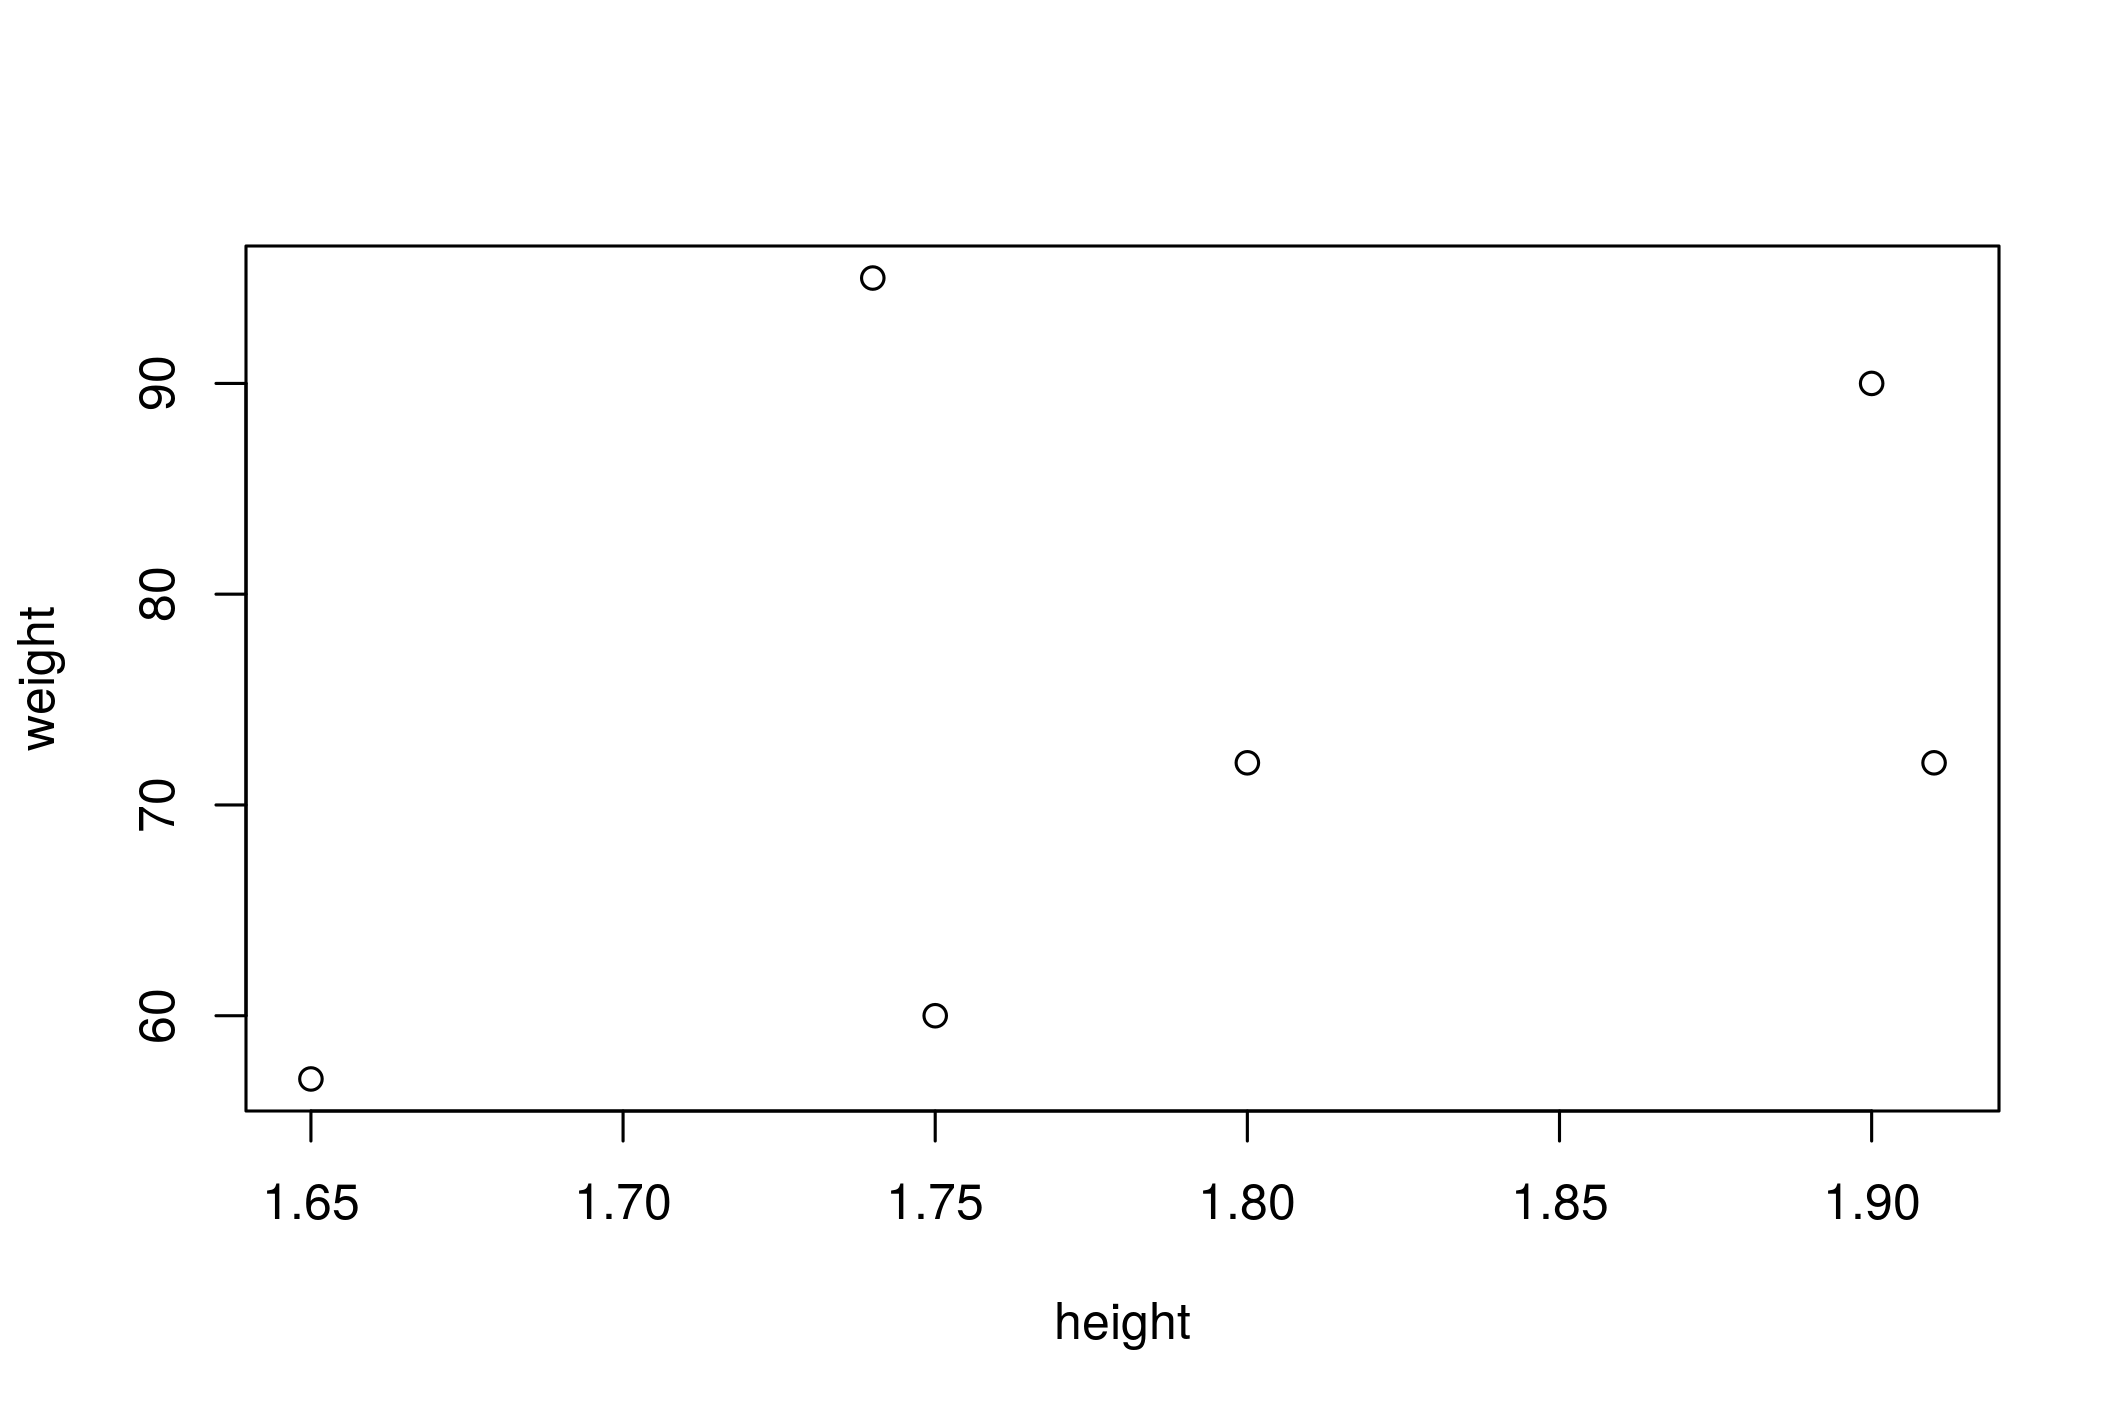
\includegraphics[width=\linewidth]{fig-2.png}
  \caption{Un simple gráfico x-y}
  \label{fig:fig-2}
\end{figure}

Puede modificar el grafico de múltiples formas. Para ello, hay una enorme
cantidad de parámetros que se pueden establecer. Como ejemplo, intentemos
cambiar el símbolo para gráficar cada punto usando la palabra clave
\texttt{pch} (``plotting character'') de esta manera:

\begin{lstlisting}[language=R]
> plot(height, weight, pch=2)
\end{lstlisting}

Esto da la gráfica en la Figura \ref{fig:fig-2}, con los puntos marcados ahora
con pequeños triángulos.

La idea detrás del cálculo del IMC es que este valor debe ser independiente de
la estatura de la persona, dando así un número único como indicación de si una
persona tiene sobrepeso y en qué medida. Dado que un IMC normal debe ser de
aproximadamente 22.5, podriamos esperar que $weight \approx 22.5 * height^2$.
De acuerdo a esto podríamos sobreponer una curva del peso esperado para un IMC
de 22.5 de la siguiente forma:

\begin{lstlisting}[language=R]
> hh <- c(1.65, 1.70, 1.75, 1.80, 1.85, 1.90)
> lines(hh, 22.5 * hh^2)
\end{lstlisting}

Lo podremos verificar en la Figura \ref{fig:fig-4}. La función \texttt{lines}
sumará los valores \texttt{(x, y))} para terminar generando una recta en el
gráfico actual.

La razón para definir una nueva variable (\texttt{hh}) para las alturas en
lugar de utilizar el vector original (\texttt{height}) es doble. En primer
lugar, la relación entre altura y peso es cuadrática y por lo tanto no lineal,
aunque puede ser difícil de ver en el gráfico. Puesto que estamos aproximando
una curva no lineal con una curva lineal a intervalos, será mejor utilizar
puntos que estén repartidos uniformemente a lo largo del eje \textit{x} que
confiar en la distribución de los datos originales. En segundo lugar, puesto
que los valores de \texttt{height} no están ordenados, los segmentos de línea
no conecta puntos vecinos, sino que se desplazan hacia adelante y hacia atrás
entre puntos distantes.

%%%%%%%%%%%%%%%%%%%%%%%%%%%%%%%%%%%%%%%%%%%%%%%%%%%%%%%%%%%%%%%%%%%%%%%%%%%%%%%
\section{R: elementos esenciales del lenguaje}
%%%%%%%%%%%%%%%%%%%%%%%%%%%%%%%%%%%%%%%%%%%%%%%%%%%%%%%%%%%%%%%%%%%%%%%%%%%%%%%

Esta sección describe los aspectos básicos del lenguaje \textbf{R}. Es
necesario hacer esto de una manera ligeramente superficial, con algunos
detalles a los que no profundizaremos demasiado.  El énfasis estará puesto en los
elementos que son útiles conocer para el uso interactivo en lugar de la
programación real , aunque se incluye una breve sección sobre programación.

%%%%%%%%%%%%%%%%%%%%%%%%%%%%%%%%%%%%%%%%%%%%%%%%%%%%%%%%%%%%%%%%%%%%%%%%%%%%%%%
\subsection{Expresiones y objetos}
%%%%%%%%%%%%%%%%%%%%%%%%%%%%%%%%%%%%%%%%%%%%%%%%%%%%%%%%%%%%%%%%%%%%%%%%%%%%%%%

La forma básica de interactuar en \textbf{R} es la de evaluación de
expresiones. El usuario introduce una expresión; el sistema la evalúa e imprime
el resultado.  Algunas expresiones se evalúan no por sus resultados sino por
los efectos secundarios tales como poner una ventana de gráficos o escribir en
un archivo. Todas las expresiones R devuelven un valor (posiblemente NULL),
pero a veces ese valor es ``invisible''  y no se imprime valor alguno en la
consola.

\newpage
\begin{figure}[!htb]
	\centering
	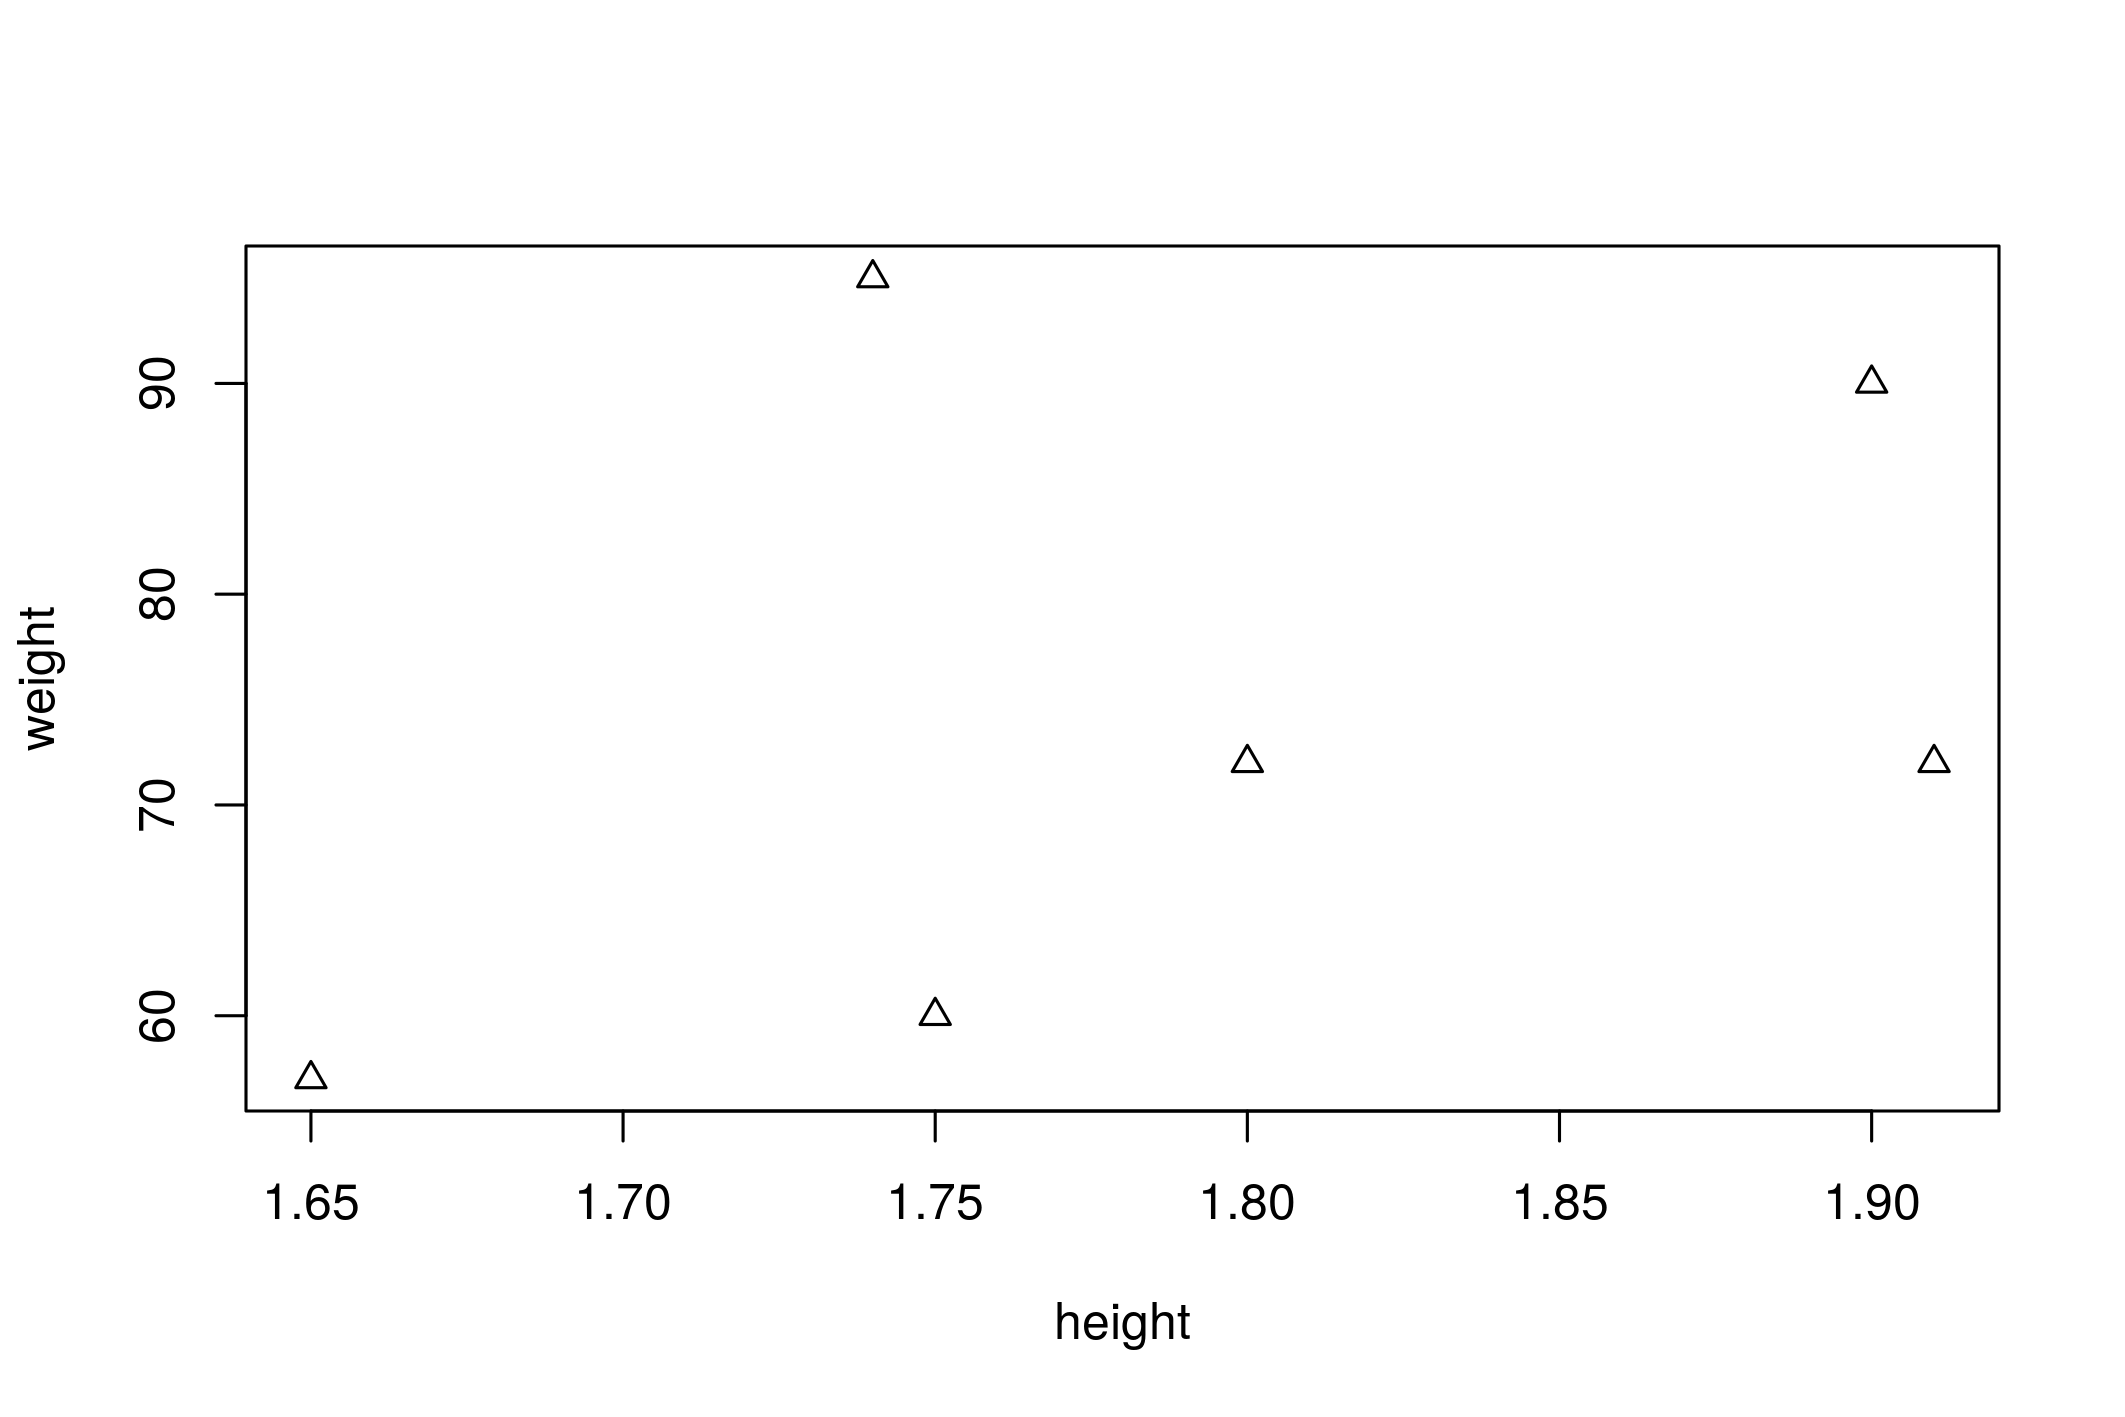
\includegraphics[width=0.95\textwidth]{fig-3.png}
	\caption{Gráfico usando \texttt{pch=2}}
	\label{fig:fig-3}
	\centering
	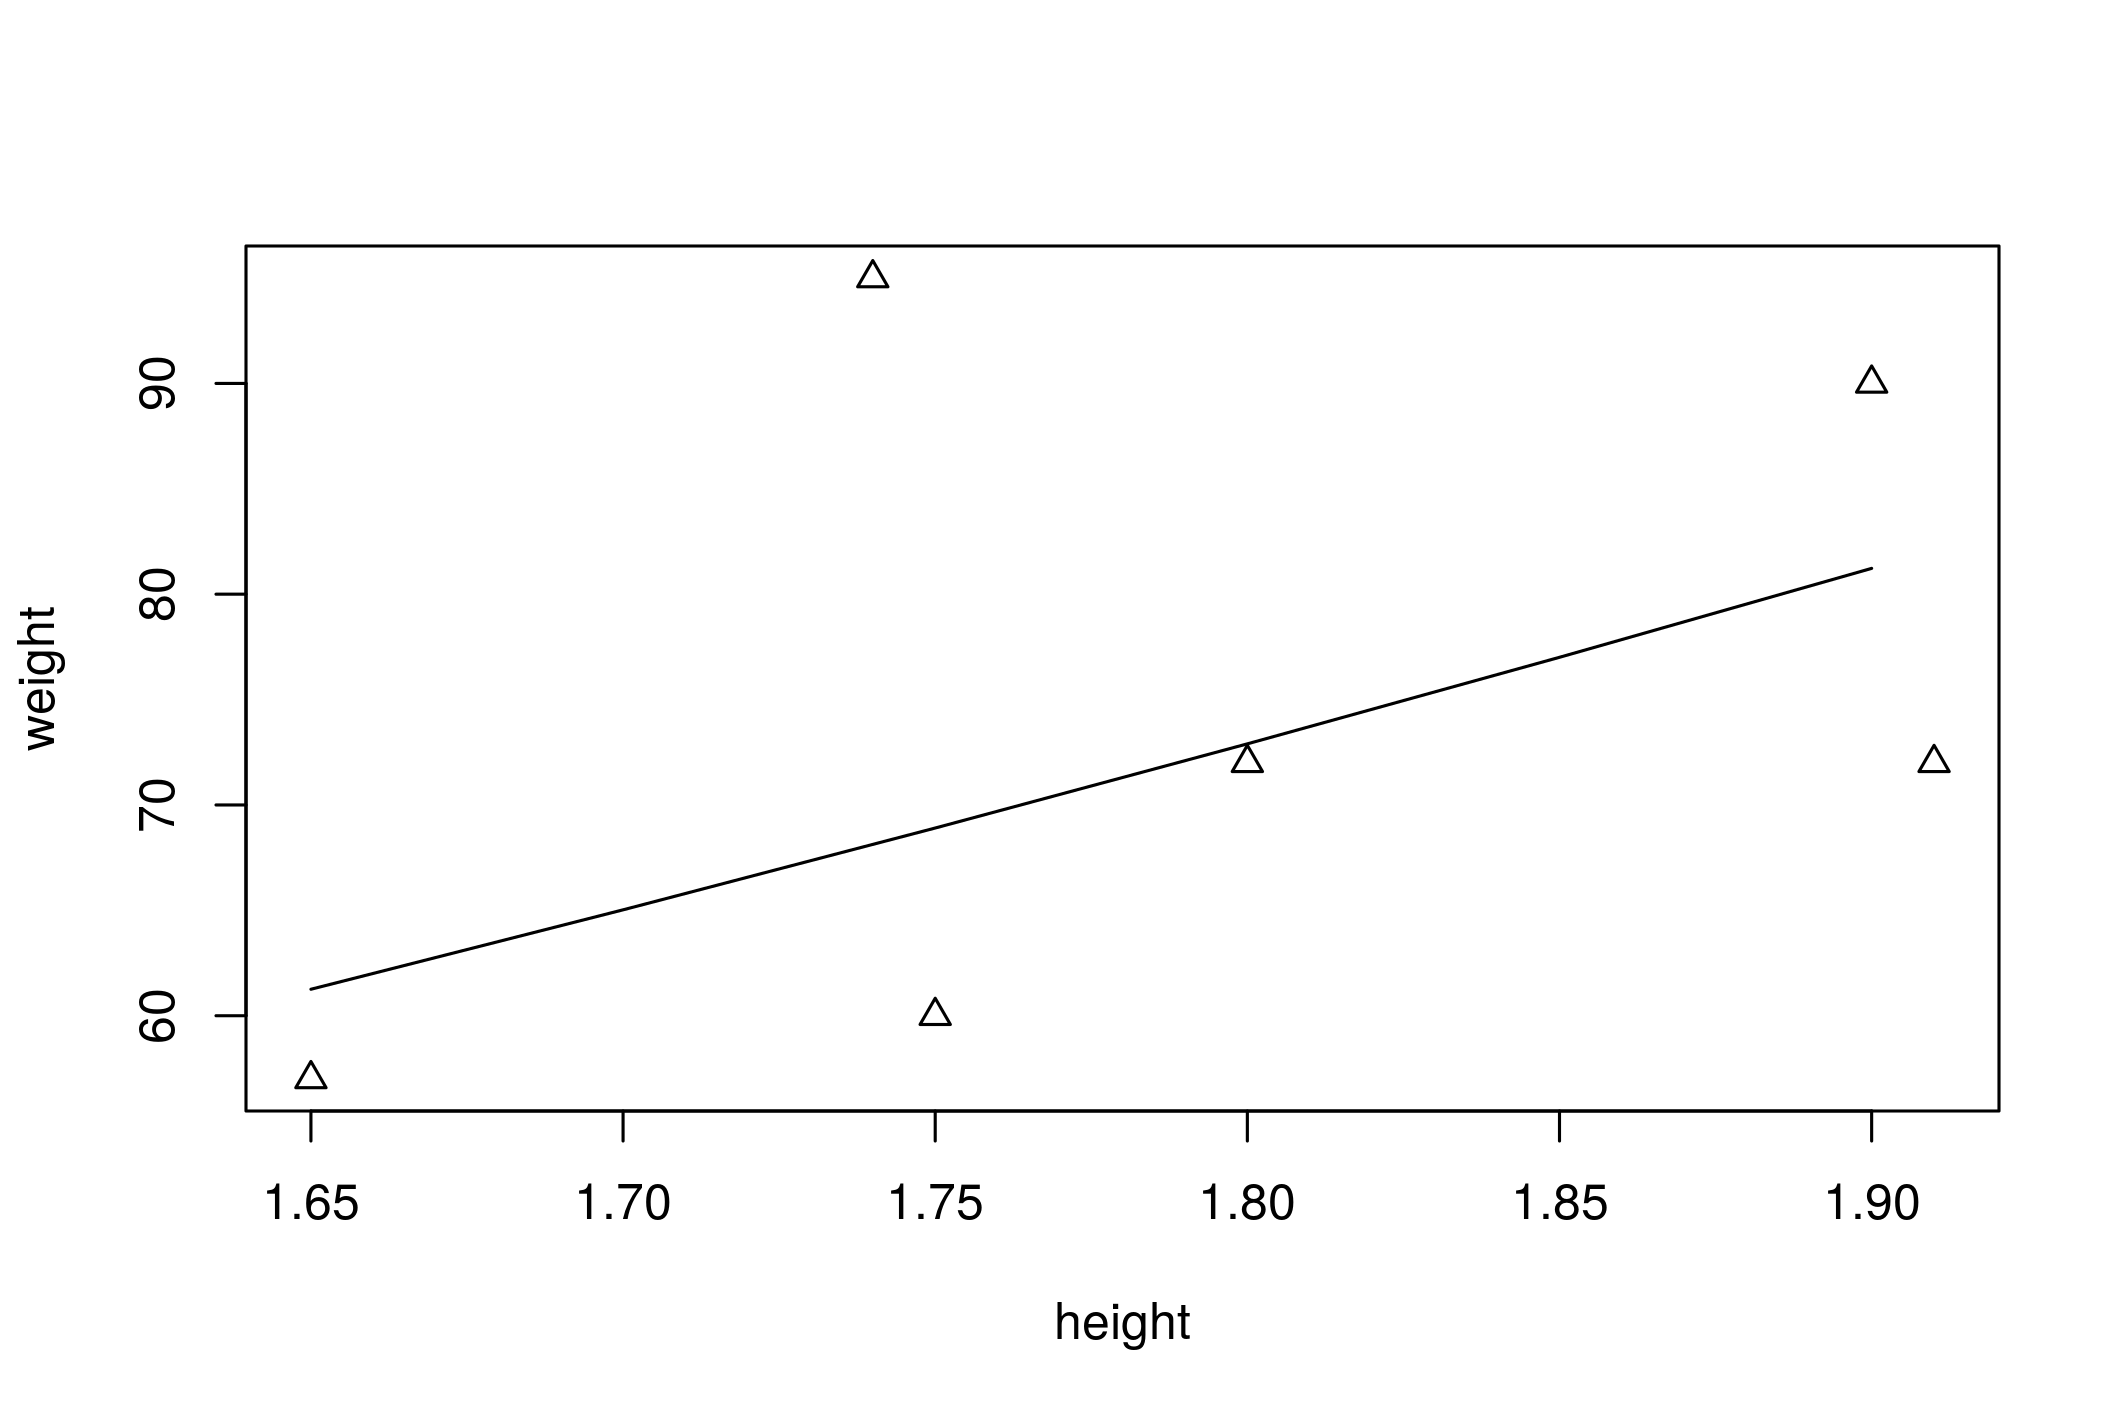
\includegraphics[width=0.95\textwidth]{fig-4.png}
	\caption{Sobreimponiendo una curva de referencia, usando \texttt{lines(...)}}
	\label{fig:fig-4}
\end{figure}
\newpage

Las expresiones suelen incluir referencias a variables, operadores como
\texttt{+} y llamadas de función, así como algunos otros elementos en los que
aún no hemos profundizado.  Las expresiones trabajan sobre objetos. Este es un
término abstracto para cualquier cosa que se pueda asignar a una variable.
\textbf{R} contiene varios tipos diferentes de objetos. Hasta ahora, hemos
visto casi exclusivamente vectores numéricos, pero en este capítulo
introduciremos varios tipos nuevos.  Aunque los objetos pueden ser explicados
de forma abstracta, sería una lectura bastante aburrida sin alguna indicación
de cómo generarlos y qué hacer con ellos. Por el contrario, gran parte de la
sintaxis de las expresiones tienen poco sentido sin conocer los objetos sobre
los que se pretende trabajar. Por lo tanto, las secciones siguientes alternan
entre la introducción de nuevos objetos y de nuevos elementos lingüísticos.

%%%%%%%%%%%%%%%%%%%%%%%%%%%%%%%%%%%%%%%%%%%%%%%%%%%%%%%%%%%%%%%%%%%%%%%%%%%%%%%
\subsection{Funciones y parámetros}
%%%%%%%%%%%%%%%%%%%%%%%%%%%%%%%%%%%%%%%%%%%%%%%%%%%%%%%%%%%%%%%%%%%%%%%%%%%%%%%

En este punto, ya tenemos una idea de la forma en que funciona \textbf{R}, y ya
hemos utilizado parte de una terminología especial cuando hablamos de la
función \texttt{plot}, etc. Ese es exactamente el punto: Muchas cosas en
\textbf{R} se hacen usando llamadas a funciones, comandos que parecen una
aplicación de una función matemática de una o varias variables; por ejemplo,
\texttt{log(x)} o \texttt{plot(height, weight)}. El formato es: un nombre de
función al cual le sigue un conjunto de paréntesis que contiene uno o más
parámetros. Por ejemplo, en \texttt{plot(height, weight)} el nombre de la
función es \texttt{plot} y los argumentos son \texttt{height} y
\texttt{weight}.  Estos son los parametros efectivos, que se usan en la
invocación final de la función, sin embargo una función también tiene
parámetros formales, que se conectan con parámetros reales en la invocación
final.

Cuando escribimos \texttt{plot(height , weight)}, \textbf{R} asume que el
primer parámetro corresponde a la variable \texttt{x} y el segundo a la
variable \texttt{y}. Esto se conoce como coincidencia posicional. Esto se
vuelve difícil de manejar si una función tiene un gran número de parámetros, ya
que hay que indicar cada uno de ellos y recordar su posición en la secuencia.
Afortunadamente, \textbf{R} tiene métodos para evitar esto: la mayoría de los
parámetros manejan valores por defecto y pueden omitirse en los casos de uso
comunes, y hay formas no posicionales de especificarlos cuando se necesita
apartarse de estos usos comunes.

La función \texttt{plot} es, de hecho, un ejemplo de una función que tiene una
gran variedad de parámetros para poder modificar símbolos, anchos de línea,
títulos, tipo de eje, etcétera. Usamos la forma alternativa de especificar
parámetros al establecer el símbolo de la gráfica en triángulos con
\texttt{plot(height, weight, pch=2)}. 

La forma \texttt{pch=2} se conoce como definición de parámetro por nombre, esta
forma permite la comparación de los parámetros de llamada con los formales de
la función y por lo tanto permite relacionar a ambos. La palabra clave
\texttt{pch} se utilizó para indicar que el parámetro corresponde con las
especificación del carácter de graficado. Esta forma de indicar cualquier
parámetro permite usar un orden arbitrario. De este modo, se puede escribir
\texttt{plot(x=height, y=weight)} y obtener el mismo gráfico que
\texttt{plot(y=weight, x=height)}.  

Los dos tipos de especificación de parámetros --posicional y por nombre-- pueden
usarse al mismo tiempo. 

Aunque no haya parámetros para el llamado a una función, es necesario escribir
\texttt{ls()}, con los paréntesis, para mostrar el contenido del espacio de
trabajo. Un error común es olvidar escribir los paréntesis, lo que termina
provocando la visualización de un trozo de código \textbf{R} puesto que
\texttt{ls} (sin paréntesis) indica que se desea ver la definición de la
función en lugar de ejecutarla.

Los parámetros formales de una función forman parte de la definición de la
misma. El conjunto de los parámetros formales de una función, por ejemplo,
\texttt{plot.default} (que es la función que se llama cuando se le pasa a
\texttt{plot} un parámetro \texttt{x} porque no existe un método especial de
trazado), puede verse con:
\newpage

\begin{lstlisting}[language=R]
> args(plot.default)
function (x, y = NULL, type = "p", xlim = NULL, ylim = NULL,
log = "", main = NULL, sub = NULL, xlab = NULL, ylab = NULL,
ann = par("ann"), axes = TRUE, frame.plot = axes,
panel.first = NULL, panel.last = NULL, asp = NA, ...)
\end{lstlisting}

Note que la mayoría de los parámetros tienen valores por defecto, en el caso de
\texttt{type} si no lo especificamos, la función se comportará como si
hubiéramos indicado \texttt{type="p"}. El \texttt{NULL} por defecto para muchos
de los parámetros, realmente sirve como indicador que el mismo no se ha
especificado, permitiendo definir un comportamiento especial dentro de la
función. Por ejemplo, si no se especifican los parámetros \texttt{xlab} e
\texttt{ylab} estos se construyen a partir de los parámetros reales pasados
como \texttt{x} e \texttt{y}. (Hay algunos puntos muy sutiles asociados con
esto, pero no vamos a profundizar más allá en el tema.)

El parámetro especial \texttt{(...)} -- Triple punto -- indica que esta función
aceptará parámetros adicionales cuyos nombres y cantidades no han sido
especificados aún de forma formal. Por lo general se usan para definir
parámetros que serán pasados a otras funciones, aunque algunas los traten de
forma particular.  Por ejemplo, en \texttt{data.frame} y \texttt{c}, los
parámetros \texttt{...} representan el resultado recibido desde otra función.

\begin{lstlisting}[language=R]
# El resultado de matrix(1:4, nrow = 2) es la entrada de data.frame(...)
> df <- data.frame(matrix(1:4, nrow = 2)) 

  X1 X2
1  1  3
2  2  4
\end{lstlisting}

%%%%%%%%%%%%%%%%%%%%%%%%%%%%%%%%%%%%%%%%%%%%%%%%%%%%%%%%%%%%%%%%%%%%%%%%%%%%%%%
\subsection{Vectores} \label{vectores}
%%%%%%%%%%%%%%%%%%%%%%%%%%%%%%%%%%%%%%%%%%%%%%%%%%%%%%%%%%%%%%%%%%%%%%%%%%%%%%%

Ya hemos visto vectores numéricos. Hay dos tipos más, vectores de caracteres y
vectores lógicos.

Un vector de caracteres es un vector de cadenas de texto cuyos elementos están
especificados entre comillas simples \texttt{'} o dobles \texttt{"}:

\begin{lstlisting}[language=R]
> c("Huey","Dewey","Louie")
[1] "Huey" "Dewey" "Louie"
\end{lstlisting}

No importa que comillas usemos, lo que es importante es que si la cadena
comienza con una finalice con la misma.

\begin{lstlisting}[language=R]
> c(\cite{Huey},\cite{Dewey}, \cite{Louie})
[1] "Huey" "Dewey" "Louie"
\end{lstlisting}

Sin embargo, debe evitar el uso del acento agudo \texttt{`}, que está presente
en algunos teclados. Usaremos las comillas dobles a lo largo de este libro para
evitar errores. Los vectores lógicos pueden tomar el valor \texttt{TRUE} o
\texttt{FALSE} (o \texttt{NA}; ver abajo). Tambien puede usar las abreviaturas
\texttt{T} y \texttt{F} (si tiene cuidado de no redefinirlas). Los vectores
lógicos se construyen usando la función \texttt{c} al igual que cualquier otros
tipo de vector:
\newpage

\begin{lstlisting}[language=R]
> c(T,T,F,T)
[1] TRUE TRUE FALSE TRUE
\end{lstlisting}

En realidad, es raro que tenga que especificar vectores lógicos de la manera
anterior. Es mucho más común usar valores lógicos únicos para activar o
desactivar una determinada opción en una llamada a una función. Los vectores de
más de un valor a menudo suelen ser el resultado de expresiones relacionales:


\begin{lstlisting}[language=R]
> bmi > 25
[1] FALSE FALSE FALSE FALSE TRUE FALSE
\end{lstlisting}

%%%%%%%%%%%%%%%%%%%%%%%%%%%%%%%%%%%%%%%%%%%%%%%%%%%%%%%%%%%%%%%%%%%%%%%%%%%%%%%
\subsection{Encomillado y secuencias de escape}
%%%%%%%%%%%%%%%%%%%%%%%%%%%%%%%%%%%%%%%%%%%%%%%%%%%%%%%%%%%%%%%%%%%%%%%%%%%%%%%

Las cadenas de caracteres entrecomilladas requieren algunas consideraciones
especiales: ¿Cómo, por ejemplo, que pasa si tenemos agregar una comilla dentro
de la cadena? ¿Y qué pasa con los caracteres especiales como el de fin de
linea? Este tipo de situaciones se resuelve usando secuencias de escape. Las
veremos inmediatamente, pero antes será útil observar lo siguiente.

Existe una diferencia entre una cadena de texto y la forma en que ésta se
imprime. Cuando, por ejemplo, se define una cadena como \texttt{"Huey"}, se
trata de una cadena de cuatro caracteres, no de seis. Las comillas no son
realmente parte de la cadena, sino que están ahí para que el sistema pueda
diferenciar entre una cadena y un nombre de variable.

Si imprime un vector de caracteres, normalmente se imprimirá con comillas
añadidas a cada elemento del mismo. Hay una manera de evitar esto, usando la
función de \texttt{cat}.  Por ejemplo,

\begin{lstlisting}[language=R]
> cat(c("Huey","Dewey","Louie"))
Huey Dewey Louie
\end{lstlisting}

Esto imprime las cadenas sin comillas, separadas por un espacio. No hay una
nueva línea que siga a la cadena, por lo que el símbolo (\texttt{>}) para la
siguiente entrada sigue directamente al final de la línea. (\textbf{Nota:}
cuando el vector de caracteres es impreso por \texttt{cat} no hay manera de
distinguir la diferencia entre este vector de tres elementos con un vector que
contuviera una simple cadena \texttt{"Huey Dewey Louie"}).

Para obtener el símbolo del sistema es necesario agregar específicamente el
caracter de salto de línea \texttt{\textbackslash{}n}

\begin{lstlisting}[language=R]
> cat(c("Huey","Dewey","Louie","\n"))
Huey Dewey Louie
>
\end{lstlisting}

Aquí hay un ejemplo de lo que se conoce como secuencia de escape. En realidad
representa un solo caracter, el linefeed (LF) o fín de línea, pero se
representa como dos caracteres. La barra invertida \textbackslash{} se conoce
como el \textit{carácter de escape}. En una forma similar, puede insertar una
comilla usando los caracteres \texttt{\"}, como en:

\begin{lstlisting}[language=R]
> cat("What is \"R\"?\n")
What is "R"?
> 
\end{lstlisting}

También hay maneras de insertar otros caracteres de control y glifos
especiales, pero nos llevaría demasiado tiempo discutirlo en detalle. Algo
importante, sin embargo: ¿Qué hay del caracter de escape en sí mismo?  Este
también debe ser escapado, así que para indicar una barra invertida, hay que
repetirla (\texttt{\textbackslash{}\textbackslash{}}). Es importante saber esto
en particular cuando cuando tengamos que especificar rutas de archivo en
Windows. Consulte también la Sección \ref{readtextfile}.

%%%%%%%%%%%%%%%%%%%%%%%%%%%%%%%%%%%%%%%%%%%%%%%%%%%%%%%%%%%%%%%%%%%%%%%%%%%%%%%
\subsection{Valores faltantes} \label{na}
%%%%%%%%%%%%%%%%%%%%%%%%%%%%%%%%%%%%%%%%%%%%%%%%%%%%%%%%%%%%%%%%%%%%%%%%%%%%%%%

En el análisis real de datos, con frecuencia no disponemos de alguna
observación (el paciente no se presentó, un experimento falló, etc.). El
software estadístico necesita formas de hacer frente a esto. \textbf{R} permite
que los vectores contengan un valor especial llamado \texttt{NA}. Este valor se
traslada a los cálculos por lo que las operaciones con valores \texttt{NA}
darán como resultado otro \texttt{NA}. Hay algunos temas especiales asociados
con el manejo de estos valores; los trataremos a medida que lo necesitemos (ver
``valores faltantes'' en el índice).

%%%%%%%%%%%%%%%%%%%%%%%%%%%%%%%%%%%%%%%%%%%%%%%%%%%%%%%%%%%%%%%%%%%%%%%%%%%%%%%
\subsection{Funciones que crean vectores}
%%%%%%%%%%%%%%%%%%%%%%%%%%%%%%%%%%%%%%%%%%%%%%%%%%%%%%%%%%%%%%%%%%%%%%%%%%%%%%%

En esta sección, presentaremos tres funciones \texttt{c}, \texttt{seq}, y
\texttt{rep}, todas se usan para crear vectores de diferentes formas.  La
primera \texttt{c}, ya la hemos visto. Es la abreviatura de ``concatenar'', que
es justamente lo que hace: juntar los elementos indicados del primero al último:

\begin{lstlisting}[language=R]
> c(42,57,12,39,1,3,4)
[1] 42 57 12 39 1 3 4
\end{lstlisting}

También podemos concatenar directamente vectores de distinta cantidad de elementos:

\begin{lstlisting}[language=R]
> x <- c(1, 2, 3)
> y <- c(10, 20)
> c(x, y, 5)
[1] 1 2 3 10 20 5
\end{lstlisting}

\begin{tradnote} Note que el vector \texttt{x} contiene 3 elementos, el vector
\texttt{y} dos, y \texttt{5} es un vector en sí mismo de un solo elemento
\end{tradnote} \newpage

De todas formas no necesitamos usar \texttt{c} para crear un vector de longitud
1. Muchos escriben \texttt{c(1)}, pero para \textbf{R} es exactamente lo mismo
que escribamos un simple \texttt{1}.

Es posible también, asignar un nombre a cada elemento de un vector. Esto
modifica luego la forma en que éste se mostrará:

\begin{lstlisting}[language=R]
> x <- c(red="Huey", blue="Dewey", green="Louie")
> x
    red    blue   green 
 "Huey" "Dewey" "Louie"
\end{lstlisting}

(En este caso si tiene sentido usar \texttt{c} incluso con vectores de un solo
elemento)

Los nombres pueden configurarse o leerse mediante la función \texttt{names}:

\begin{lstlisting}[language=R]
> names(x)
[1] "red"   "blue"  "green"
\end{lstlisting}

En el caso de los vectores, todos los elementos deben ser del mismo tipo. Si
concatenamos diferentes tipos de datos \textbf{R} convertira todos al tipo menos
restrictivo:

\begin{lstlisting}[language=R]
> c(FALSE, 3)
[1] 0 3
> c(pi, "abc")
[1] "3.14159265358979" "abc"
> c(FALSE, "abc")
[1] "FALSE" "abc"
\end{lstlisting}

Lo que ocurrió es, que los valores lógicos se convierten a valores \texttt{0/1}
o \texttt{"FALSE/TRUE"} y los números a una representación de tipo cadena.

La segunda función, \texttt{seq}("secuencia"), se usa para generar series de
números equidistantes. Al escribir esto:

\begin{lstlisting}[language=R]
> seq(4,9)
[1] 4 5 6 7 8 9
\end{lstlisting}

Podemos ver claramente, que hemos creado un vector con los enteros del 4 al 9.
Si buscamos secuencias que "salten" de a 2 elementos, podríamos escribir:

\begin{lstlisting}[language=R]
> seq(4,10,2)
[1] 4 6 8 10
\end{lstlisting}

Frecuentemente son necesarios estos tipos de vectores, particlarmente para
gráficos. Por ejemplo, anteriormente usamos un vector
\texttt{c(1.65,1.70,1.75,1.80,1.85,1.90)} para definir un conjunto de alturas,
algo que eventualmente podríamos haber escrito como
\texttt{seq(1.65,1.90,0.05)} (La ventaja de usar \texttt{seq} es más que obvia
si eventualmente necesitaramos crear pasos de 1cm en vez de 5cm)

Una forma especial de definir una secuencia con pasos igual a 1 es la siguiente:

\begin{lstlisting}[language=R]
> 4:9
[1] 4 5 6 7 8 9
\end{lstlisting}

Lo anterior es exactamente igual a hacer \texttt{seq(4,9)}, simplemente es más
sencillo de leer.

La tercer función, \texttt{rep} ("replicar"), es usada para generar valores que
se repiten. Se puede usar de dos formas, dependiendo si el segundo parámetro es
un vector o un número

\begin{lstlisting}[language=R]
> oops <- c(7,9,13)
> rep(oops,3)
[1]  7  9 13  7  9 13  7  9 13
> rep(oops,1:3)
[1]  7  9  9 13 13 13
\end{lstlisting}

La primera de las ejecuciones repite completamente el vector \texttt{oops} tres
veces.  La segunda llamada repite cada elemento la cantidad de veces definida
en el segundo vector \texttt{(1,2,3)}, es decir que el 7 se repetirá una vez,
el 9 dos, y el 13 tres.

La función \texttt{rep} se usa habitualmente para hacer cosas como agrupar elementos: Si
sabemos que las primeras 10 observaciones son hombres y las últimas 17 mujeres,
podemos hacer:

\begin{lstlisting}[language=R]
> rep(1:2,c(10,15))
[1] 1 1 1 1 1 1 1 1 1 1 2 2 2 2 2 2 2 2 2 2 2 2 2 2 2
\end{lstlisting}

Para armar un vector que nos indica que las observaciones corresponden a un
hombre (1) o a una mujer (2).  Una forma de repetir un mismo número de veces un
elemento, puede lograrse mediante \texttt{rep(1:2,each=10)} que es lo mismo que
hacer \texttt{rep(1:2,c(10,10))}.

%%%%%%%%%%%%%%%%%%%%%%%%%%%%%%%%%%%%%%%%%%%%%%%%%%%%%%%%%%%%%%%%%%%%%%%%%%%%%%%
\subsection{Matrices y arreglos}
%%%%%%%%%%%%%%%%%%%%%%%%%%%%%%%%%%%%%%%%%%%%%%%%%%%%%%%%%%%%%%%%%%%%%%%%%%%%%%%

En matemáticas, una matriz no es más que una arreglo de números de dos
dimensiones. Se usan muchísimo en las estadísticas teóricas y prácticas, pero
en este libro no asumimos que el lector este familiarizado con el álgebra de
las matrices, por lo que evitaremos explicar muchas de las operaciones
específicas como el producto escalar (El documento "An Introduction to R", que
acompaña a la instalación, describe estos puntos bastante bien). Sin embargo,
las matrices y los arreglos de más de una dimensión también se utilizan para
propósitos más simples, principalmente para manejar tablas, por lo que una
descripción elemental es necesaria. En \textbf{R}, la noción de matriz se
extiende a elementos de cualquier tipo, por lo cual podríamos tener, por
ejemplo, una matriz de cadenas de caracteres. Las matrices y los arreglos se
representan como vectores con dimensiones:


\begin{lstlisting}[language=R]
> x <- 1:12
> dim(x) <- c(3,4)
> x
[,1] [,2] [,3] [,4]
[1,] 1 4 7 10
[2,] 2 5 8 11
[3,] 3 6 9 12
\end{lstlisting}

En el ejemplo anterior, la función \texttt{dim()} establece las dimensiones de
la matriz \texttt{x}, hace que \textbf{R} convierta un vector de 12 números en
una matriz de 3 x 4. Observe que la asignación se hace en el orden de las
columnas, los tres primeros números representan la primer columna, los números
4 al 6, la segunda y así hasta el final.

Una forma conveniente de crear matrices es utilizando la función \texttt{matrix()}:

\begin{lstlisting}[language=R]
matrix(1:12,nrow=3,byrow=T)
     [,1] [,2] [,3] [,4]
[1,]    1    2    3    4
[2,]    5    6    7    8
[3,]    9   10   11   12
\end{lstlisting}

Notese que al usar el parámetro \texttt{byrow=T} hacemos que la matriz se
complete por fila en vez del modo habitual por columna.

Hay función muy útiles que pueden operar sobre las matrices como
\texttt{rownames()}, \texttt{colnames()} y la funcion de transponer
\texttt{t()} que transforma filas a columnas y visceversa (tome note que el
nombre esta en minúscula al contrario de \texttt{T} que representa el valor
\texttt{Verdadero}).

\begin{tradnote} Es importante mencionar, aunque se verá más adelante, que
estas funciones no se restringen solo a las matrices sino que aplican a
múltiples estructuras similares a estas.\end{tradnote} \newpage

\begin{lstlisting}[language=R]
> x <- matrix(1:12,nrow=3,byrow=T)
> rownames(x) <- LETTERS[1:3]
> x
  [,1] [,2] [,3] [,4]
A    1    2    3    4
B    5    6    7    8
C    9   10   11   12
> t(x)
     A B  C
[1,] 1 5  9
[2,] 2 6 10
[3,] 3 7 11
[4,] 4 8 12
\end{lstlisting}

El vector de caracteres \texttt{LETTERS} es una variable ya definida en
\textbf{R}, que contine todas las letras en mayúsculas (en el alfabeto inglés
eso sí). También existen otros vectores similares muy útiles como
\texttt{letters}, \texttt{month.name} o \texttt{month.abb} que contienen,
letras en minúsculas, el nombre de los meses y los nombres de los meses en modo
abreviado respectivamente.

Es posible "pegar" vectores entre sí, en forma de columnas o filas, utilizando
las funciones \texttt{cbind} y \texttt{rbind} (``column bind'' y ``row bind'').

\begin{lstlisting}[language=R]
cbind(A=1:4,B=5:8,C=9:12)
     A B  C
[1,] 1 5  9
[2,] 2 6 10
[3,] 3 7 11
[4,] 4 8 12
> rbind(A=1:4,B=5:8,C=9:12)
  [,1] [,2] [,3] [,4]
A    1    2    3    4
B    5    6    7    8
C    9   10   11   12
\end{lstlisting}

Volveremos a las operaciones tabulares en la Sección \ref{tables}.

\subsection{Factores}

Es habitual en los datos estadísticos tener variables categóricas, que indican
algún tipo de subdivisión, como ser clase social, diagnóstico primario, estadio
tumoral, etapa de la pubertad de Tanner, etc. Normalmente estos datos se
trabajan como algún tipo de código numérico. 

Sin embargo en \textbf{R} podemos definir estas variables como
\textit{Factores}, un tipo de estructura, que entre otras cosas, permite
asignar un nombre descriptivo a estas categorías.  

Hay ciertos análisis dónde es esencial para \textbf{R} distinguir
entre estos códigos categóricos y variables cuyos valores tienen un significado
numérico directo (véase el capítulo 7). 

Un factor tiene un conjunto de niveles, digamos 4 como ejemplo, internamente un
factor de 4 niveles esta constituido por: (a) un vector de números enteros de 1
a 4 y (b) un vector de caracteres de longitud 4 que contiene las cadenas que
describen cuales son estos cuatro niveles. Veamos un ejemplo:

\begin{lstlisting}[language=R]
> pain <- c(0,3,2,2,1)
> fpain <- factor(pain,levels=0:3)
> levels(fpain) <- c("none","mild","medium","severe")
\end{lstlisting}

El primer comando crea un vector numérico llamado \texttt{pain} que codifica el
nivel de dolor de 5 pacientes. Trataremos de manejar esto como una variable
categórica, entonces creamos un factor que llamamos \texttt{fpain} usando
justamente la función \texttt{factor()}. Esta es llamada con un parámetro
adicional a \texttt{pain}, \texttt{levels=0:3}, lo que indica que la
codificación usa los valores 0 a 3.

Podríamos haber obviado el indicar el parámetro \texttt{levels}, ya que \textbf{R} usa
los mismos valores de \texttt{pain} en el orden adecuado, sin embargo es una buena
práctica hacerlo. El resultado final se ve claramente:

\begin{lstlisting}[language=R]
> fpain
[1] none   severe medium medium mild  
Levels: none mild medium severe
> as.numeric(fpain)
[1] 1 4 3 3 2
> levels(fpain)
[1] "none" "mild" "medium" "severe"
\end{lstlisting}

La función \texttt{as.numeric} recupera la codificación numérica: 1-4 y
\texttt{levels} recupera los nombre de cada nivel. Observe que la codificación
original de 0 a 3 ha desaparecido, esto es por que la representación interna de
un \texttt{factor} siempre comienza por 1. 

\begin{tradnote} De hecho, todos los objetos en \textbf{R} se indizan a partir de 1, a
diferencia de otros lenguajes como \textbf{C} dónde el índice inicial es el
0.\end{tradnote}

\textbf{R} también le permite crear un tipo especial de factor en el que los
niveles se mantienen ordenados.  Esto se logra usando la función
\texttt{ordered} que funciona de una forma similar a \texttt{factor}.  Esto es
potencialmente útil ya que podemos distinguir entre variables nominales y
ordinales (se podría decir que el factor anterior debería haber sido un factor
ordenado) Desafortunadamente, \textbf{R} por defecto trata los niveles como si
fueran equidistantes en el código de modelado (generando contrastes
polinomiales), por lo que es mejor ignorar los factores ordenados por ahora.

%%%%%%%%%%%%%%%%%%%%%%%%%%%%%%%%%%%%%%%%%%%%%%%%%%%%%%%%%%%%%%%%%%%%%%%%%%%%%%%
\subsection{Listas} \label{listas}
%%%%%%%%%%%%%%%%%%%%%%%%%%%%%%%%%%%%%%%%%%%%%%%%%%%%%%%%%%%%%%%%%%%%%%%%%%%%%%%

En algunos casos es útil combinar una colección de objetos en un único objeto
compuesto. Esto lo podemos lograr usando las \textit{listas}. 

Podemos construir una lista a partir de los objetos individuales que la
conformarán, usando la función \texttt{list}.

Como ejemplo, considere un conjunto de datos de Altman (1991, p. 183) sobre la
ingesta de energía pre y postmenstrual en un grupo de mujeres. Podemos colocar
estos datos en dos vectores como sigue:

\begin{lstlisting}[language=R]
> intake.pre <- c(5260,5470,5640,6180,6390,
+ 6515,6805,7515,7515,8230,8770)
> intake.post <- c(3910,4220,3885,5160,5645,
+ 4680,5265,5975,6790,6900,7335)
\end{lstlisting}

Observe como podemos continuar de escribir las sentencias en la linea
siguiente. Si presionamos la tecla Enter cuando la sentencia es sintácticamente
incompleta, \textbf{R} asume que la expresión continua en la siguiente línea y el
símbolo habitual > cambia por el +. Esto puede suceder de forma inadvertida
debido, por ejemplo, a la falta de un paréntesis, o algún caso semejante; en
esos casos, o bien se completa la expresión en la línea siguiente o se puede
presionar la tecla ESC (Windows and Macintosh) o Ctrl-C (Unix). En windows
también podremos usar el botón ``Stop''. 

Para combinar los dos vectores anteriores en una lista:

\begin{lstlisting}[language=R]
> mylist <- list(before=intake.pre,after=intake.post)
> mylist
$before
[1] 5260 5470 5640 6180 6390 6515 6805 7515 7515 8230 8770
$after
[1] 3910 4220 3885 5160 5645 4680 5265 5975 6790 6900 7335
\end{lstlisting}

Los componentes de una lista puede nombrarse de acuerdo a los nombres de los
parámetros indicados en al invocar a \texttt{list}. Los componentes de la lista
que han sido nombrados pueden recuperarse de la siguiente forma:

\begin{lstlisting}[language=R]
> mylist$before
[1] 5260 5470 5640 6180 6390 6515 6805 7515 7515 8230 8770
\end{lstlisting}

Muchas de las funciones de \texttt{R} que pueden retornar más de un valor lo
hacen por medio de listas.

%%%%%%%%%%%%%%%%%%%%%%%%%%%%%%%%%%%%%%%%%%%%%%%%%%%%%%%%%%%%%%%%%%%%%%%%%%%%%%%
\subsection{Data frames}
%%%%%%%%%%%%%%%%%%%%%%%%%%%%%%%%%%%%%%%%%%%%%%%%%%%%%%%%%%%%%%%%%%%%%%%%%%%%%%%

Un \textit{data frame} corresponde a lo que otros paquetes estadísticos llaman
una ``matriz de datos'' o un ``conjunto de datos''. Es una lista de vectores y/o
factores de la misma longitud que están relacionados "horizontalmente" de tal manera
que los datos en la misma fila corresponden a la misma unidad experimental
(sujeto, animal, etc.). Además, tiene un conjunto único de nombres de filas.

Podemos crear un \texttt{data.frame} con los datos del ejemplo anterior:

\begin{lstlisting}[language=R]
> d <- data.frame(intake.pre,intake.post)
> d
   intake.pre intake.post
1        5260        3910
2        5470        4220
3        5640        3885
4        6180        5160
5        6390        5645
6        6515        4680
7        6805        5265
8        7515        5975
9        7515        6790
10       8230        6900
11       8770        7335
\end{lstlisting}

Note que estos datos están ``emparejados'', es decir, la misma mujer tiene una
ingesta de 5260 kJ premenstrualmente y 3910 kJ postmenstrualmente.

De igual forma que las listas, lo componentes o variables individuales pueden
ser accedidos usando la notación \texttt{\$}:

\begin{lstlisting}[language=R]
> d$intake.pre
[1] 5260 5470 5640 6180 6390 6515 6805 7515 7515 8230 8770
\end{lstlisting}

%%%%%%%%%%%%%%%%%%%%%%%%%%%%%%%%%%%%%%%%%%%%%%%%%%%%%%%%%%%%%%%%%%%%%%%%%%%%%%%
\subsection{Indexado} \label{index}
%%%%%%%%%%%%%%%%%%%%%%%%%%%%%%%%%%%%%%%%%%%%%%%%%%%%%%%%%%%%%%%%%%%%%%%%%%%%%%%

En caso de necesitar acceder a un elemento en particular de un vector, por
ejemplo la ingesta premenstrual para la mujer número 5 , podemos hacer:

\begin{lstlisting}[language=R]
> intake.pre[5]
[1] 6390
\end{lstlisting}

Los corchetes se utilizan para la selección de datos, también conocido como
acceso por índice o extración de un subcojunto (indexing o subsetting en
inglés). Esto funciona también del lado izquierdo de la asignación (por lo que
por ejemplo podríamos hacer \texttt{intake.pre[5] <- 6390}) si quisieramos
modificar uno de los elemento del vector.

Si queremos otro vector compuesto de los datos de más de una de las mujeres,
por ejemplo la 3, 5 y 7, podemos hacer lo siguiente:

\begin{lstlisting}[language=R]
> intake.pre[c(3,5,7)]
[1] 5640 6390 6805
\end{lstlisting}

Observe que es necesario el uso de la función \texttt{c(...)} para definir un
vector que contenga los números 3, 5 y 7. \texttt{intake.pre[3,5,7]} significa
algo completamente distinto, una operación de acceso por índice de un vector de
tres dimensiones.

Por supuesto, el acceso por índice también funciona si el vector de selección
viene definido en una variable. Esto es útil si queremos repetir la misma
operación de selección en mmúltiples conjuntos de datos.

\begin{lstlisting}[language=R]
> v <- c(3,5,7)
> intake.pre[v]
[1] 5640 6390 6805
> intake.post[v]
[1] 3885 5645 5265
\end{lstlisting}

Tampoco reviste ningún problema recuperar una secuencia de elementos, por
ejemplo los primeros 5, para esto usaremos la notación \texttt{a:b}:

\begin{lstlisting}[language=R]
> intake.pre[1:5]
[1] 5260 5470 5640 6180 6390
\end{lstlisting}


Una característica muy interesante de \textbf{R} es la posibilidad de usar
índices negativos, para negar una cierta selección. Podemos recuperar todas
las observaciones \textit{excepto} la 3,5 y 7:

\begin{lstlisting}[language=R]
> intake.pre[-c(3,5,7)]
[1] 5260 5470 6180 6515 7515 7515 8230 8770
\end{lstlisting}

Lo que no podemos es combinar índices negativos y positivos ya que esto trae
aparejado una ambiguedad eventualmente imposible de manejar.

%%%%%%%%%%%%%%%%%%%%%%%%%%%%%%%%%%%%%%%%%%%%%%%%%%%%%%%%%%%%%%%%%%%%%%%%%%%%%%%
\subsection{Selección condicional}
%%%%%%%%%%%%%%%%%%%%%%%%%%%%%%%%%%%%%%%%%%%%%%%%%%%%%%%%%%%%%%%%%%%%%%%%%%%%%%%

Ya vimos en la sección \ref{index}, como extraer dados usando uno o más
índices. En la práctica, lo más habitual es seleccionar datos que cumplan con
un cierto criterio, como como los datos de aquellas observaciones
correspondientes a varones, o a los prepúberes o a los que padecen enfermedades
crónicas, etc. Esto se puede hacer simplemente insertando una expresión
relacional en lugar del índice,

\begin{lstlisting}[language=R]
> intake.post[intake.pre > 7000]
[1] 5975 6790 6900 7335
\end{lstlisting}

Esto recupera aquellas casos de mujeres dónde la ingesta de energía
postmenstrual está por encima de 7000 kJ premenstrualmente.

Este tipo de expresión tiene sentido siempre que la expresión relacional opere
sobre la misma cantidad de registros que la variable indexada.

Los operadores de comparación disponibles, son similares a lo que podemos tener
en cualquier otro lenguaje, por ejmplo \textbf{C} y son: < (menor a), > (mayor
a), == (igual a), <= (menor o igual a), >= (mayor o igual a), y != (distinto).
Es importante notar que el test de igualdad usa el doble igual (==), esto es
para evitar confusión con el simple = que usamos para la asignación de
parámetros en una función, o eventualmente en la asignación de valores a una
variable.

Para combinar varias expresiones, podemos usar los operadores lógicos \& (y
lógico), | (o lógico) y ! (no lógico). Por ejemplo para ubicar los casos de
ingesta postmenstrual en mujeres dónde la ingesta premenstrual se encuentra
comprendida entre los 7000 y 8000 Kj, podemos hacer:

\begin{lstlisting}[language=R]
> intake.post[intake.pre > 7000 & intake.pre <= 8000]
[1] 5975 6790
\end{lstlisting}

Existen también los operadores \&\& y ||, los cuales se usan para el control de
flujo en la programación en \textbf{R}. De todas formas su utilidad esta fuera
del alcance en esta etapa.  Cale la pena prestar atención a lo que realmente
sucede cuando usamos una expresión lógica como índice. El resultado termina
siendo un vector lñogico tal como lo hemos secripto en la sección
\ref{vectores}, 

\begin{lstlisting}[language=R]
> intake.pre > 7000 & intake.pre <= 8000
[1] FALSE FALSE FALSE FALSE FALSE FALSE FALSE TRUE TRUE FALSE
[11] FALSE
\end{lstlisting}

La selección por índice por medio de un vector lógico significa que tomaremos
los valores dónde el vector lógico sea Verdadero. En el ejemplo anterior
recuperaremos el valor octavo y noveno de \texttt{intake.post}.

Si hubiera valores faltantes (\texttt{NA}, como vimos en la sección \ref{na})
en el vector lógico, \textbf{R} completará el valor correspondiente con el
valor \texttt{NA}.

Además de de los operadores lógicos y relacionales, tenemos una serie de
funciones que retornan un valor lógico. Es particularmente importante
\texttt{is.na(x)}, que se usa justamente para determinar que elementos de
\texttt{x} son \texttt{NA}.

Es importante tener claro que existe una necesidad muy concreta para
\texttt{is.na(x)}, no es posible hacer comparaciones del tipo \texttt{x == NA},
esto simplemente retornará un valor \texttt{NA}. El resultado de la comparación
con un valor desconocido es otro valor desconocido.

%%%%%%%%%%%%%%%%%%%%%%%%%%%%%%%%%%%%%%%%%%%%%%%%%%%%%%%%%%%%%%%%%%%%%%%%%%%%%%%
\subsection{Indexado de data frames}
%%%%%%%%%%%%%%%%%%%%%%%%%%%%%%%%%%%%%%%%%%%%%%%%%%%%%%%%%%%%%%%%%%%%%%%%%%%%%%%

Ya hemos visto que podemos extraer variables de un \texttt{data.frame},
ingresando, por ejemplo, \texttt{d\$intake.post}. De cualquier forma, es
posible también usar una notación que aprovecha la estructura matricial del
\texttt{data.frame}:

\begin{lstlisting}[language=R]
> d <- data.frame(intake.pre,intake.post)
> d[5,1]
[1] 6390
\end{lstlisting}

Esto nos daría el valor ubicado en la quinta fila y la primer columna, que
representa la medida previa de la mujer número 5 y,

\begin{lstlisting}[language=R]
> d[5,]
  intake.pre intake.post
5       6390        5645
\end{lstlisting}

nos devolverá las medidas completas para la mujer número 5. Note que se
requiere usar la coma en \texttt{d[5,]}, sin ésta, por ejemplo \texttt{d[2]},
obtendríamos un \texttt{data.frame} compuesto únicamente por la segunda columna
(que es como si hiciéramos \texttt{d[,2]}, que es la columna en sí misma).

Pero también podemos aplicar otras técnicas de selección o indexado, puede ser
útil obtener todos los casos que satisfacen algún criterio, como por ejemplo,
las mujeres cuya ingesta premestrual fue superior a los 7000 kJ:

\begin{lstlisting}[language=R]
> d[d$intake.pre>7000,]
   intake.pre intake.post
8        7515        5975
9        7515        6790
10       8230        6900
11       8770        7335
\end{lstlisting}

Para entender exactamente lo que hemos hecho, vamos a dividirlo en pasos más
pequeños:

\begin{lstlisting}[language=R]
> sel <- d$intake.pre>7000
> sel
 [1] FALSE FALSE FALSE FALSE FALSE FALSE FALSE  TRUE  TRUE  TRUE  TRUE

> d[sel,]
   intake.pre intake.post
8        7515        5975
9        7515        6790
10       8230        6900
11       8770        7335
\end{lstlisting}

Lo que ha pasado es que hemos definido \texttt{sel} como un vector lógico,
dónde el valor \texttt{TRUE} se corresponden con las 4 mujeres con más de 7000
kJ de ingesta premestrual.

Ahora, al hacer \texttt{d[sel,]} seleccionamos aquellas filas de \texttt{d} que
correspondan a los valores \texttt{TRUE} de \texttt{sel}, y por supuesto, todas
las columnas ya que dejamos vacío es lugar luego de la coma.

Muchas veces es conveniente ver los primeros casos de un juego de datos. Esto
puede hacerse mediante el indexado o selección, de esta forma:

\begin{lstlisting}[language=R]
> d[1:2,]
  intake.pre intake.post
1       5260        3910
2       5470        4220
\end{lstlisting}

Esto se suele hacer tan a menudo que ya existe la función \texttt{head}. Por
defecto nos traera los primeros 6 elementos.

\begin{lstlisting}[language=R]
> head(d)
  intake.pre intake.post
1       5260        3910
2       5470        4220
3       5640        3885
4       6180        5160
5       6390        5645
6       6515        4680
\end{lstlisting}

De forma similar, existe la función \texttt{tail} para mostrarnos los últimos
elementos.

%%%%%%%%%%%%%%%%%%%%%%%%%%%%%%%%%%%%%%%%%%%%%%%%%%%%%%%%%%%%%%%%%%%%%%%%%%%%%%%
\subsection{Agrupación de datos y data frames}
%%%%%%%%%%%%%%%%%%%%%%%%%%%%%%%%%%%%%%%%%%%%%%%%%%%%%%%%%%%%%%%%%%%%%%%%%%%%%%%

La forma más natural de almacenar grupos de datos en un \texttt{data.frame} es tener
los mismos en un solo vector y paralelamente, tener un factor que
indique a que grupo pertenece. Considere, por ejemplo, el siguiente
conjunto de datos sobre el gasto de energía para las mujeres delgadas y obesas.

\begin{lstlisting}[language=R]
> energy
   expend stature
1    9.21   obese
2    7.53    lean
3    7.48    lean
4    8.08    lean
5    8.09    lean
6   10.15    lean
7    8.40    lean
8   10.88    lean
9    6.13    lean
10   7.90    lean
11  11.51   obese
12  12.79   obese
13   7.05    lean
14  11.85   obese
15   9.97   obese
16   7.48    lean
17   8.79   obese
18   9.69   obese
19   9.68   obese
20   7.58    lean
21   9.19   obese
22   8.11    lean
\end{lstlisting}

Esta forma es muy conveniente ya que permite fácilmente clasificar los datos
por múltiples criterios.  De todas formas, en ocasiones, puede ser deseable
separar en distintos vectores cada uno de los grupos, lo cual es muy sencillo de
hacer:

\begin{lstlisting}[language=R]
> exp.lean <- energy$expend[energy$stature=="lean"]
> exp.obese <- energy$expend[energy$stature=="obese"]
\end{lstlisting}

Y de una forma más generalizable podemos usar la función \texttt{split} que generará una
lista de vectores de acuerdo a los grupos existentes.

\begin{lstlisting}[language=R]
> l <- split(energy$expend, energy$stature)
> l
$lean
 [1]  7.53  7.48  8.08  8.09 10.15  8.40 10.88  6.13  7.90  7.05  7.48  7.58  8.11

$obese
[1]  9.21 11.51 12.79 11.85  9.97  8.79  9.69  9.68  9.19
\end{lstlisting}

%%%%%%%%%%%%%%%%%%%%%%%%%%%%%%%%%%%%%%%%%%%%%%%%%%%%%%%%%%%%%%%%%%%%%%%%%%%%%%%
\subsection{Ciclos implícitos}\label{ciclosimplicitos}
%%%%%%%%%%%%%%%%%%%%%%%%%%%%%%%%%%%%%%%%%%%%%%%%%%%%%%%%%%%%%%%%%%%%%%%%%%%%%%%

La construcción de ciclos en \textbf{R} se describen en la Sección \ref{flowcontrol}.
Para los propósitos de este libro, podemos ignorar en gran medida la existencia
de estos. Sin embargo, hay un grupo de funciones \textbf{R} que será útil conocer.

Un uso muy común de un ciclo es el de aplicar una función a cada elemento de un
conjunto de valores o vectores y recoger los resultados en una sola estructura.
En \textbf{R} esto se logra mediante el uso de las funciones \texttt{lapply} y
\texttt{sapply}. La primera siempre devuelve una lista (de ahí la \texttt{l}),
mientras que la segunda intenta simplificar (de ahí la \texttt{s}) el resultado
a un vector o a una matriz si es posible. Por lo tanto, para calcular la media
de cada variable en un \texttt{data.frame} con valores numéricos, podríamos hacer lo
siguiente

\begin{lstlisting}[language=R]
> lapply(thuesen, mean, na.rm=T)
$blood.glucose
[1] 10.3

$short.velocity
[1] 1.325652

> sapply(thuesen, mean, na.rm=T)
 blood.glucose short.velocity 
     10.300000       1.325652 
\end{lstlisting}

Observe que ambas funciones dotaron a los resultados de un nombre informativo,
lo cual es otra razón para usar estas funciones en vez de los ciclos
explicítos. El segundo parámetro to \texttt{lapply/sapply} es el nombre de la
función que se aplicará , en este caso \texttt{mean}. 

Cualquier otro parámetro se pasa a la función a continuación; en este caso
pasamos \texttt{na.rm=T} para indicar que se eliminen los valores faltantes
(ver \ref{resestad}).  A veces sólo queremos repetir algo un número de veces
pero aún así guardar los resultados en un vector. Obviamente, esto tiene
sentido sólo cuando los cálculos repetitivos dan resultados diferentes, siendo
el caso común los estudios de simulación. Esto se puede hacer usando
\texttt{sapply}, pero hay una versión simplificada llamada \texttt{replicate},
en el que sólo tienes que dar un recuento y la expresión a evaluar:

\begin{lstlisting}[language=R]
> replicate(10,mean(rexp(20)))
 [1] 0.8369313 0.9651302 1.0437885 0.7174850 0.8586701 0.5218970 1.5854871
 [8] 1.1025462 0.9269089 1.3222753
\end{lstlisting}

Una función similar, \texttt{apply}, nos permite "aplicar" un determinada
función a las filas o columnas de una matriz (o sobre los índices de cualquier
arreglo multidimensional)

\begin{lstlisting}[language=R]
> m <- matrix(rnorm(12),4)
> m
           [,1]       [,2]        [,3]
[1,] -0.2007822  2.0034906 -0.44432912
[2,]  1.3281647 -1.2074197  0.06629581
[3,]  2.2353936 -0.1198466 -1.82850943
[4,]  0.3476552  1.2306042  0.34204225
> apply(m, 2, min)
[1] -0.2007822 -1.2074197 -1.8285094
\end{lstlisting}

El segundo parámetro en este caso es el índice (o vector de índices) que define
a qué se aplica la función; en este caso calculamos los mínimos por columna.
Además, tenemos la función \texttt{tapply} que permite crear tablas (de ahí la
\texttt{t}) del valor de una función en subgrupos definidos por su segundo
parámetro, que puede ser un factor o una lista de factores. En este último
caso, se genera una tabla de clasificación cruzada. (La agrupación también
puede ser definida por vectores ordinarios que internamente se convertirán a
factores.)

\begin{lstlisting}[language=R]
> tapply(energy$expend, energy$stature, median)
 lean obese 
 7.90  9.69 
\end{lstlisting}

%%%%%%%%%%%%%%%%%%%%%%%%%%%%%%%%%%%%%%%%%%%%%%%%%%%%%%%%%%%%%%%%%%%%%%%%%%%%%%%
\subsection{Orden}
%%%%%%%%%%%%%%%%%%%%%%%%%%%%%%%%%%%%%%%%%%%%%%%%%%%%%%%%%%%%%%%%%%%%%%%%%%%%%%%

Es trivial ordenar un vector, simplemente usaremos la función \texttt{sort}.
(Aprovecharemos los datos \texttt{intake}; contiene la misma información que
usamos en la sección \ref{listas})

\begin{lstlisting}[language=R]
> intake$post
 [1] 3910 4220 3885 5160 5645 4680 5265 5975 6790 6900 7335
> sort(intake$post)
 [1] 3885 3910 4220 4680 5160 5265 5645 5975 6790 6900 7335
\end{lstlisting}

(No podemos usar \texttt{intake\$pre} en este ejemplo por que ya se encuentra
ordenada!)

Sin embargo, el orden de un solo vector no siempre es lo que se
requiere. A menudo es necesario ordenar una serie de variables de acuerdo con
los valores de algunas otras variables - presiones sanguíneas ordenadas por
sexo y edad, por ejemplo. Para este propósito, hay una construcción que puede
parecer algo abstracta al principio pero que es realmente muy poderosa. Primero
se calcula el orden de una variable.

\begin{lstlisting}[language=R]
> order(intake$post)
 [1]  3  1  2  6  4  7  5  8  9 10 11
\end{lstlisting}

El resultado son los números del 1 al 11 (o cualquiera que sea la longitud del
vector), ordenados de acuerdo al valor del parámetro a ordenar (aquí
\texttt{intake\$post}). Interpretar el resultado de \texttt{order} es un poco
complicado - debe leerse de la siguiente manera: Usted ordena \texttt{intake\$post}
ubicando sus valores en el orden no. 3, no. 1, no. 2, no. 6, etc.

El punto es, que este vector puede servir para ordenar otras variables usando
el mismo criterio. Tenga en cuenta que la indización con un vector que contiene
los números del 1 al número exacto de elementos corresponde a una reordenación
de estos.

\begin{lstlisting}[language=R]
> o <- order(intake$post)
> intake$post[o]
 [1] 3885 3910 4220 4680 5160 5265 5645 5975 6790 6900 7335
> intake$pre[o]
 [1] 5640 5260 5470 6515 6180 6805 6390 7515 7515 8230 8770
\end{lstlisting}


Lo que ocurrió aquí es que hemos ordenado \texttt{intake\$post}, mientras que
\texttt{intake\$pre} fue ordenada también pero según el orden de los valores de
\texttt{intake\$post}. Es posible ordenar directamente el data frame
\texttt{intake}

\begin{lstlisting}[language=R]
> intake.sorted <- intake[o,]
\end{lstlisting}

Ordenar por múltiples criterios es tan sencillo como indicar las variables a
usar como parámetros de la función \texttt{order}; por ejemplo
\texttt{order(sex, age}, ordenará primero por sexo y luego dentro de cada
grupo, por la edad. El orden descendente se puede establecer modificando el
signo de la variable

%%%%%%%%%%%%%%%%%%%%%%%%%%%%%%%%%%%%%%%%%%%%%%%%%%%%%%%%%%%%%%%%%%%%%%%%%%%%%%%
\section{Ejercicios}
%%%%%%%%%%%%%%%%%%%%%%%%%%%%%%%%%%%%%%%%%%%%%%%%%%%%%%%%%%%%%%%%%%%%%%%%%%%%%%%

1.1 ¿Cómo verificarías si dos vectores son iguales si contienen valores
faltantes (\texttt{NA})? (usar la función \texttt{identical()} es hacer
trampa!

1.2 Si \texttt{x} es un \texttt{factor} con \texttt{n} niveles e \texttt{y} es
un vector con longitud \texttt{n}, ¿que sucede si hacemos \texttt{y[x]}?

1.3 Escriba una expresión lógica para obtener las mujeres entre 7 y 14 años del
conjunto de datos \texttt{juul}

1.4 ¿Que ocurre si modificamos los niveles de un \texttt{factor} (con la
función \texttt{levels()}) con los mismos niveles más dos o más niveles?

1.5 En la página \pageref{ciclosimplicitos}, usamos \texttt{replicate} para
generar 10 números que se corrresponden con la media de una distribución
exponenecial.  ¿Cómo podríamos conseguir lo mismo usando \texttt{sapply}?

%%%%%%%%%%%%%%%%%%%%%%%%%%%%%%%%%%%%%%%%%%%%%%%%%%%%%%%%%%%%%%%%%%%%%%%%%%%%%%%
%% El Entorno de R
%%%%%%%%%%%%%%%%%%%%%%%%%%%%%%%%%%%%%%%%%%%%%%%%%%%%%%%%%%%%%%%%%%%%%%%%%%%%%%%
\chapter{El entorno de R}

Este capítulo comprende algunos aspectos prácticos del trabajo con \textbf{R}.
Describe cuestiones relacionadas con la estructura del espacio de trabajo, los
dispositivos gráficos y sus parámetros, y la programación elemental, e incluye
una discusión bastante extensa, aunque lejos de ser completa, sobre el ingreso
de datos.

%%%%%%%%%%%%%%%%%%%%%%%%%%%%%%%%%%%%%%%%%%%%%%%%%%%%%%%%%%%%%%%%%%%%%%%%%%%%%%%
\section{Administración de sesiones}
%%%%%%%%%%%%%%%%%%%%%%%%%%%%%%%%%%%%%%%%%%%%%%%%%%%%%%%%%%%%%%%%%%%%%%%%%%%%%%%

%%%%%%%%%%%%%%%%%%%%%%%%%%%%%%%%%%%%%%%%%%%%%%%%%%%%%%%%%%%%%%%%%%%%%%%%%%%%%%%
\subsection{El espacio de trabajo}
%%%%%%%%%%%%%%%%%%%%%%%%%%%%%%%%%%%%%%%%%%%%%%%%%%%%%%%%%%%%%%%%%%%%%%%%%%%%%%%

Todas las variables creadas en R se almacenan en un espacio de trabajo común.
Para ver qué variables están definidas en el área de trabajo, puede utilizar la
función \texttt{ls} (lista).  Si ha ejecutado todos los ejemplos del capítulo
anterior es posible que la salida sea similar a esto:

\begin{lstlisting}[language=R]
> ls()
 [1] "bmi"           "d"             "exp.lean"      "exp.obese"    
 [5] "fpain"         "height"        "hh"            "intake.post"  
 [9] "intake.pre"    "intake.sorted" "l"             "m"            
[13] "mylist"        "o"             "oops"          "pain"         
[17] "sel"           "v"             "weight"        "x"            
[21] "xbar"          "y"   
\end{lstlisting}

Recuerde no omitir los paréntesis al invocar a \texttt{ls}().

Si en algún momento las cosas comienzan a ser confusas, podemos eliminar
algunos objetos del entorno. Esto se puede hacer mediante \texttt{rm}()
(remover), de manera que:

\begin{lstlisting}[language=R]
> rm(height, weight)
\end{lstlisting}

Elimina las variables \texttt{height} y \texttt{weight}.

Se puede eliminar completamente el espacio de trabajo mediante
\texttt{rm(list=ls())}, y también mediante la opciones de menú “Remove all
objects” o “Clear Workspace” en las versiones graficas de \textbf{R}. Esto no
elimina las variables cuyo nombre comienza con un punto (\texttt{.}) por que
las mismas no son listadas por \texttt{ls()} - necesitaríamos usa
\texttt{ls(all=T)} para eso,  pero podría ser peligros ya que algunos objetos
usados por el sistema usan esta notación.

Si está familiarizado con el sistema operativo \textbf{Unix}, para el cual el
lenguaje \textbf{S}, que precedió a \textbf{R}, fue escrito originalmente,
entonces sabrá que los comandos para listar y eliminar archivos en Unix se
llaman precisamente \texttt{ls} y \texttt{rm}.

Es posible salvar completamente el espacio de trabajo en cualquier momento.
Simplemente deberemos escribir:

\begin{lstlisting}[language=R]
> save.image()
\end{lstlisting}

de esta forma, todo será salvado en un archivo de nombre \texttt{.RData} en el
directorio de trabajo actual. Las versiones gráficas también tienen un menú
para hacer esto. Cuando salimos de \textbf{R} se nos puede llegar a preguntar
si queremos salvar una imagen de nuestro espacio de trabajo; si le decimos que
sí estaremos haciendo exactamente lo mismo. Es posible también especificar un
nombre de archivo a salvar alternativo (usando comillas), también podremos
salvar objetos específicos con \texttt{save}. El archivo \texttt{.RData} se
carga automáticamente cuando se inicia \texttt{R} desde el directorio dónde se
encuentre. Otros archivos similares pueden cargarse al espacio de trabajo
mediante \texttt{load}.

%%%%%%%%%%%%%%%%%%%%%%%%%%%%%%%%%%%%%%%%%%%%%%%%%%%%%%%%%%%%%%%%%%%%%%%%%%%%%%%
\subsection{Salida Textual}
%%%%%%%%%%%%%%%%%%%%%%%%%%%%%%%%%%%%%%%%%%%%%%%%%%%%%%%%%%%%%%%%%%%%%%%%%%%%%%%

Es importante tener en cuenta que el espacio de trabajo está formado únicamente
por objetos \textbf{R}, no por ninguna de las salidas generadas durante la
sesión de trabajo.  Si desea guardar ésta utilice "Guardar en archivo" en el
menú Archivo de la versión Gráfica o utilice las funciones estándar de cortar y
pegar. También puede utilizar \textbf{ESS} (Emacs Speaks Statistics), que
funciona en todas las plataformas. Es un "modo" para el editor \textbf{Emacs}
en el que puede ejecutar toda la sesión en un búfer. Puede obtener la
\textbf{ESS} y las instrucciones de instalación de \textbf{CRAN} (ver Apéndice
A).  

Una forma alternativa de redirigir la salida a un archivo es usar la función
\texttt{sink}. Se trata en gran medida de una reliquia de la época de las
terminales de 80 x 25, en la que no se disponía de técnicas de cortar y pegar,
pero que aún puede ser útil en ocasiones. En particular, se puede utilizar en
el procesamiento por lotes. La forma en que funciona es de la siguiente manera:

\begin{lstlisting}[language=R]
> sink("salidatxt")
> ls()
\end{lstlisting}

No aparece ninguna salida por pantalla!. Esto por que ahora la salida normal de
cualquier comando o función se redirige automáticamente al archivo
\texttt{salida.txt} en el directorio actual.  El sistema permanecerá trabajando
de esta forma hasta que ejecutemos nuevamente (esta vez sin parámetros):

\begin{lstlisting}[language=R]
> sink()
\end{lstlisting}

El directorio de trabajo actual se puede obtener mediante \texttt{getwd()} y
establecer otro mediante \texttt{setwd(mi directorio)}, dónde \texttt{mi
directorio} es una cadena de texto. El directorio de trabajo inicial depende
del sistema, por ejemplo para las versiones gráficas suele ser el \texttt{home
dir} del usuario y en la versión de línea de comandos es la carpeta desde dónde
se ha ejecutado \textbf{R}.

%%%%%%%%%%%%%%%%%%%%%%%%%%%%%%%%%%%%%%%%%%%%%%%%%%%%%%%%%%%%%%%%%%%%%%%%%%%%%%%
\subsection{Scripting}
%%%%%%%%%%%%%%%%%%%%%%%%%%%%%%%%%%%%%%%%%%%%%%%%%%%%%%%%%%%%%%%%%%%%%%%%%%%%%%%

Más allá de un cierto nivel de complejidad, seguramente no querrá trabajar con
\textbf{R} línea por línea. En estas situaciones, es mejor trabajar con scripts
\textbf{R}, colecciones de líneas de código almacenadas en un archivo o en la
memoria de la computadora de alguna forma. 

Una opción es usar la función de \texttt{source}, que es algo así como lo
opuesto a \texttt{sink}. Toma la entrada (es decir, los comandos desde un
archivo) y los ejecuta. Nótese, sin embargo, que todo el archivo se comprueba
sintácticamente antes de que ejecutar cualquier instrucción. A menudo es útil
configurar \texttt{echo=T} en la llamada para que los comandos sean impresos
junto con la salida. 

Otra opción es de naturaleza más interactiva. Puedes trabajar con un editor que
le permite enviar una o más líneas del script a una instancia de R en
ejecución, el cual se comportará como si las mismas líneas hubieran sido
introducida en el indicador de comandos. Las versiones de Windows, Linux y
Macintosh de R tienen ventanas de scripting simples incorporadas, y un número
importante de Editores de texto tienen la funcionalidad para enviar los
comandos a R.

\begin{tradnote} 
	
	Actualmente son muchas las herramientas para trabajar en R, muchas más de
	las que existían al momento de la publicación original de este libro. En
	lineas generales hoy tenemos R en las tres principales plataformas:
	Windows, Linux y MAC, en cada una además podemos contar con:

	\begin{description}
	\item[$\bullet$] Interprete interactivo por línea de comando (\texttt{R})
	\item[$\bullet$] Versión grafica (\texttt{Rgui})
	\item[$\bullet$] Múltiples editores de texto con integración con \textbf{R}
	\item[$\bullet$] Entornos integrados de desarrollo (\textbf{Rstudio})
	\end{description}

\end{tradnote}

El historial de los comandos introducidos en una sesión se puede guardar y
volver a cargar utilizando los comandos \texttt{savehistory} y
\texttt{loadhistory}, que también se asignan a entradas de menú en la versión
gráfica. Las comandos guardados pueden ser útiles como punto de partida para
escribir scripts; observe también que la función \texttt{history()} mostrará
los últimos comandos introducidos en la consola (hasta un máximo de 25 líneas
por defecto)

%%%%%%%%%%%%%%%%%%%%%%%%%%%%%%%%%%%%%%%%%%%%%%%%%%%%%%%%%%%%%%%%%%%%%%%%%%%%%%%
\subsection{El sistema de ayuda de R}
%%%%%%%%%%%%%%%%%%%%%%%%%%%%%%%%%%%%%%%%%%%%%%%%%%%%%%%%%%%%%%%%%%%%%%%%%%%%%%%

\textbf{R} puede hacer mucho más de lo que un principiante podría llegar a
necesitar o incluso entender. Este libro está escrito de tal manera que la
mayor parte del código que probablemente necesitará en relación con los
procedimientos estadísticos se describe en el texto, y el compendio en el
Apéndice C está diseñado para proporcionar una visión general básica. Sin
embargo, es evidente que no es posible abarcar todo.  

\textbf{R} también viene con una amplia ayuda en línea en forma de texto, así
como en forma de una serie de archivos HTML que se pueden leer utilizando
cualquier navegador Web Se puede acceder a las páginas de ayuda a través de
``help'' en la barra de menú de Windows e introduciendo \texttt{help.start()} en
cualquier plataforma. Encontrará que las páginas son de naturaleza técnica. La
precisión y la concisión prevalecen aquí sobre la legibilidad y la pedagogía
(algo que se aprende a apreciar después de la exposición a lo contrario).  

Desde la línea de comandos, siempre puede introducir \texttt{help(aggregate)}
para obtener ayuda de la función \texttt{aggregate} o utilizar el prefijo
\texttt{?}, por ejemplo: \texttt{?aggregate}. Si el visor de HTML se está
ejecutando, entonces la página de ayuda se mostrará allí. De lo contrario, se
mostrará como texto en un misma ventana del terminal o en una ventana separada.
Tenga en cuenta que la versión HTML del sistema de ayuda incluye un ``Motor de
búsqueda y claves'' muy útil y que la función \texttt{apropos} le permite
obtener una lista de nombres de comandos que contienen un patrón dado. La
función \texttt{help.search} es similar, pero utiliza coincidencias difusas y
busca más profundamente en las páginas de ayuda, de modo que podrá localizar,
por ejemplo, el coeficiente de correlación de Kendall en \texttt{cor.test} si
utiliza \texttt{help.search("kendal")}. 

También está disponible con las distribuciones de \textbf{R}, un conjunto de
documentos en varios formatos. Es particularmente interesante ``An Introduction
to R'', basado originalmente en una serie de notas para \textbf{S-PLUS} de Bill
Venables y David Smith y adaptado a \textbf{R} por varias personas.  Contiene
una introducción al lenguaje \textbf{R} y al entorno, mucho más centrada en el
lenguaje en sí que este libro. En la plataforma Windows, puede elegir instalar
documentos PDF como parte del procedimiento normal de instalación para poder
acceder luego por medio del menú ``Ayuda''.  Se puede acceder también a una
versión HTML (sin imágenes) a través del navegador en todas las plataformas.

%%%%%%%%%%%%%%%%%%%%%%%%%%%%%%%%%%%%%%%%%%%%%%%%%%%%%%%%%%%%%%%%%%%%%%%%%%%%%%%
\subsection{Paquetes}\label{paquetes}
%%%%%%%%%%%%%%%%%%%%%%%%%%%%%%%%%%%%%%%%%%%%%%%%%%%%%%%%%%%%%%%%%%%%%%%%%%%%%%%

Una instalación de \texttt{R} contiene una o más librerías o paquetes. Algunos
de estos paquetes forman parte de la instalación básica.  Otros pueden ser
descargados desde \textbf{CRAN} (ver apéndice A), el cual alberga a la fecha
más de 12000 paquetes para múltiples propósitos.  Incluso podríamos crear
nuestros propios paquetes. Una librería es por lo general una simple carpeta en
el disco. Una librería de sistema se crea al instalar \texttt{R}.  En algunas
instalaciones, no les es permitido a los usuarios modificar la librería del
sistema. De todas formas, es posible configurara librerías privadas; para más
detalles ver \texttt{help(".Library")}.

Un paquete puede contener, funciones escritas en \textbf{R}, librerías de carga
dinámica escritas en \textbf{C} o \textbf{Fortran} y distintos conjuntos de
datos.  Un paquete generalmente implementa funcionalidad que la mayoría de los
usuarios probablemente no necesiten tener cargada todo el tiempo. Un paquete es
cargado en \textbf{R} mediante el comando \texttt{library}, de esta forma, para
cargar el paquete \texttt{survival} tendremos que ingresar:

\begin{lstlisting}[language=R]
> library(survival)
\end{lstlisting}

Los paquetes cargados, no se consideran parte del espacio de trabajo. Si
terminamos la sesión \texttt{R} y comenzamos una nueva con es espacio de
trabajo guardado, deberemos cargar nuevamente los paquetes anteriores.  Por
esta misma razón, rara vez necesitemos descargar un paquete activo, pero si lo
llegaremos a necesitar hacer, podríamos escribir:

\begin{lstlisting}[language=R]
> detach("package:survival")
\end{lstlisting}

(ver sección \ref{attachdetach}.)

%%%%%%%%%%%%%%%%%%%%%%%%%%%%%%%%%%%%%%%%%%%%%%%%%%%%%%%%%%%%%%%%%%%%%%%%%%%%%%%
\subsection{Datos integrados}
%%%%%%%%%%%%%%%%%%%%%%%%%%%%%%%%%%%%%%%%%%%%%%%%%%%%%%%%%%%%%%%%%%%%%%%%%%%%%%%

Muchos paquetes, tanto dentro como fuera de la distribución R estándar, vienen
con algún que otro conjunto de datos incorporado. Estos conjuntos de datos
pueden ser bastante grandes, por lo que no es una buena idea mantenerlos en la
memoria en todo momento. Se requiere entonces, un mecanismo para la carga bajo
demanda. En muchos paquetes, esto funciona a través de un mecanismo llamado
\textit{carga perezosa} ("lazy loading,"), que permite al sistema "simular" que
los datos están sí  en memoria, pero en realidad no se cargan hasta que son
referenciados por primera vez.  

Con este mecanismo, los datos están al alcance de la mano. Por ejemplo, si
escribe \texttt{thuesen}, se muestra el \texttt{data.frame} de dicho nombre.
Algunos paquetes todavía requieren llamadas explícitas a la función
\texttt{data}.  La mayoría de las veces, esto carga un \texttt{data.frame} con
el nombre que se especifica como parámetro; \texttt{data(thuesen)}, por
ejemplo, carga el \texttt{data.frame} "thuesen".

Lo que hace \texttt{data} es recorrer los directorios de datos asociados a cada
paquete (ver Sección \ref{paquetes}) y buscar archivos cuyo nombre base
coincida con el nombre especificado. Dependiendo de la extensión del archivo,
pueden suceder varias cosas. Los archivos con extensión \texttt{.tab} se leen
usando \texttt{read.table} (Sección \ref{readtextfile}), mientras que los
archivos con extensión \texttt{.R} se ejecutan como archivos de código (¡y
podrían, en general, hacer cualquier cosa!), esto simplemente, por dar dos
ejemplos comunes.

Si hay un subdirectorio del directorio actual llamado \texttt{data}, entonces
también se busca en él. Esta puede ser una forma muy útil de organizar sus
proyectos personales.

%%%%%%%%%%%%%%%%%%%%%%%%%%%%%%%%%%%%%%%%%%%%%%%%%%%%%%%%%%%%%%%%%%%%%%%%%%%%%%%
\subsection{\texttt{attach} y \texttt{detach}}\label{attachdetach}
%%%%%%%%%%%%%%%%%%%%%%%%%%%%%%%%%%%%%%%%%%%%%%%%%%%%%%%%%%%%%%%%%%%%%%%%%%%%%%%

La notación para acceder a variables en \texttt{data.frames} se vuelve bastante pesada
si tiene que escribir repetidamente comandos largos como:

\begin{lstlisting}[language=R]
> plot(thuesen$blood.glucose,thuesen$short.velocity)
\end{lstlisting}

Afortunadamente, puede hacer que\textbf{R} busque objetos entre las variables
de un \texttt{data.frame} determinado, por ejemplo \texttt{thuesen}. Escribiendo:

\begin{lstlisting}[language=R]
> attach(thuesen)
\end{lstlisting}

y entonces los datos de \texttt{thuesen} estarán disponibles sin la engorrosa
notación \texttt{\$}:

\begin{lstlisting}[language=R]
> blood.glucose
 [1] 15.3 10.8  8.1 19.5  7.2  5.3  9.3 11.1  7.5 12.2  6.7  5.2
[13] 19.0 15.1  6.7  8.6  4.2 10.3 12.5 16.1 13.3  4.9  8.8  9.5
\end{lstlisting}

Lo que sucedió aquí es que el \texttt{data.frame} \texttt{thuesen} se colocan en la
ruta de búsqueda del sistema. Puede ver la misma con el comando:

\begin{lstlisting}[language=R]
> search()
 [1] ".GlobalEnv"        "thuesen"           "package:ISwR"     
 [4] "tools:rstudio"     "package:stats"     "package:graphics" 
 [7] "package:grDevices" "package:utils"     "package:datasets" 
[10] "package:methods"   "Autoloads"         "package:base"     
\end{lstlisting}

Nótese que \texttt{thuesen} se coloca en segundo lugar en la ruta de búsqueda.
\texttt{.GlobalEnv} es el espacio de trabajo y \texttt{package:base} es la
biblioteca del sistema donde se definen todas las funciones estándar. Omitimos
describir \texttt{Autoloads}.  \texttt{package:stats} en adelante contiene las
rutinas estadísticas básicas como el test de Wilcoxon, y los otros paquetes
contienen de forma similar varias funciones y conjuntos de datos. (El sistema
de paquetes es modular, y puede ejecutar \textbf{R} con un conjunto mínimo de
paquetes para usos específicos. Por último, \texttt{package:ISwR} contiene los
conjuntos de datos utilizados para este libro. 


Puede haber varios objetos del mismo nombre en diferentes partes de la ruta de
búsqueda. En ese caso, \textbf{R} elige la primera (es decir, busca primero en
\texttt{.GlobalEnv}, luego en \texttt{thuesen}, y así sucesivamente). Por esta
razón, hay que tener un poco de cuidado con los objetos "sueltos" que se
definen en el espacio de trabajo fuera de un \texttt{data.frame}, ya que se
utilizarán antes que cualquier vector y factor del mismo nombre en el 
\texttt{data.frame} específico. Por la misma razón, no es una buena idea dar a
un \texttt{data.frame} el mismo nombre que a una de las variables dentro de él.
Tenga en cuenta también que cambiar un \texttt{data.frame} después de
adjuntarlo no afectará a las variables disponibles a partrir del
\texttt{attach}, ya que adjuntar implica una operación de copia (virtual) del
\texttt{data.frame} 

No es posible adjuntar \texttt{data.frame} antes de \texttt{.GlobalEnv} o después de
\texttt{package:base}. Sin embargo, es posible adjuntar más de un \texttt{data.frame}. Las
nuevos \texttt{data.frame} se insertan en la posición 2 de forma predeterminada, y
todo excepto \texttt{.GlobalEnv} se mueve un paso a la derecha. Sin embargo, es posible
especificar que se debe buscar un marco de datos antes de \texttt{.GlobalEnv} utilizando
construcciones de la forma de:

\begin{lstlisting}[language=R]
> with(thuesen, plot(blood.glucose, short.velocity))
\end{lstlisting}

En algunos contextos, \textbf{R} usa un método ligeramente diferente para
buscar objetos. Si se busca una variable de un tipo específico (generalmente
una función), \textbf{R} omitirá las de otros tipos. Esto ahorra las peores
consecuencias de nombrar accidentalmente una variable, por ejemplo \texttt{c},
aunque exista una función del sistema con el mismo nombre.

Puede eliminar un \texttt{data.frame} de la ruta de búsqueda con
\texttt{detach}. Si no se dan argumentos, el \texttt{data.frame} en la posición
2 se elimina, que es generalmente lo que se desea. \texttt{.GlobalEnv} y \texttt{package:base} no
se pueden desadjuntar (\texttt{detach}) del entorno. 

\begin{lstlisting}[language=R]
> detach()
> search()

 [1] ".GlobalEnv"        "package:ISwR"      "tools:rstudio"    
 [4] "package:stats"     "package:graphics"  "package:grDevices"
 [7] "package:utils"     "package:datasets"  "package:methods"  
[10] "Autoloads"         "package:base"    
\end{lstlisting}

%%%%%%%%%%%%%%%%%%%%%%%%%%%%%%%%%%%%%%%%%%%%%%%%%%%%%%%%%%%%%%%%%%%%%%%%%%%%%%%
\subsection{subset, transform, y within}
%%%%%%%%%%%%%%%%%%%%%%%%%%%%%%%%%%%%%%%%%%%%%%%%%%%%%%%%%%%%%%%%%%%%%%%%%%%%%%%

Puede adjuntar un \texttt{data.frame} para evitar la engorrosa indexación de cada
variable dentro de él. Sin embargo, esto es poco práctico para seleccionar
subconjuntos de datos y para crear nuevos \texttt{data.frame} con variables
transformadas. Existen un par de funciones para facilitar estas operaciones. Se
utilizan de la siguiente manera:

\begin{lstlisting}[language=R]
> thue2 <- subset(thuesen,blood.glucose<7)
> thue2

   blood.glucose short.velocity
6            5.3           1.49
11           6.7           1.25
12           5.2           1.19
15           6.7           1.52
17           4.2           1.12
22           4.9           1.03

> thue3 <- transform(thuesen,log.gluc=log(blood.glucose))
> thue3 

   blood.glucose short.velocity log.gluc
1           15.3           1.76 2.727853
2           10.8           1.34 2.379546
3            8.1           1.27 2.091864
4           19.5           1.47 2.970414
5            7.2           1.27 1.974081
...
22           4.9           1.03 1.589235
23           8.8           1.12 2.174752
24           9.5           1.70 2.251292
\end{lstlisting}

Note que las variables usadas en las expresiones para crear nuevas variables o
para construir subconjunto son evaluadas con variables del propio
\texttt{data.frame}.

\texttt{subset} también funciona con vectores individuales. Esto es casi lo
mismo que la indexación con un vector lógico (como ser
\texttt{short.velocity[blood.glucose<7]}), excepto que se excluyen las
observaciones con valores faltanantes (\texttt{NA}) en el criterio de
selección.

\texttt{subset} también tiene un parámetros \texttt{select} que puede usarse
para extraer variables del \texttt{data.frame}. Volveremos sobre esto en la
sección \label{appending frames}.

La función de \texttt{transform} tiene un par de inconvenientes, el más grave,
probablemente sea, que no permite cálculos encadenados donde algunas de las
nuevas variables dependen de las otras. Los signos \texttt{=} en la sintaxis no
son asignaciones, sino que indican nombres, que se asignan a los vectores
calculados en el último paso.

Una alternativa a \texttt{transform} es la función \texttt{within}, que puede
ser utilizada de esta manera:

\begin{lstlisting}[language=R]
> thue4 <- within(thuesen,{
        log.gluc <- log(blood.glucose)
        m <- mean(log.gluc)
        centered.log.gluc <- log.gluc - m
        rm(m)
})

> thue4
   blood.glucose short.velocity centered.log.gluc log.gluc
1           15.3           1.76       0.481879807 2.727853
2           10.8           1.34       0.133573113 2.379546
3            8.1           1.27      -0.154108960 2.091864
4           19.5           1.47       0.724441444 2.970414
5            7.2           1.27      -0.271891996 1.974081
...
22           4.9           1.03      -0.656737817 1.589235
23           8.8           1.12      -0.071221300 2.174752
24           9.5           1.70       0.005318777 2.251292
\end{lstlisting}

Note que el segundo parámetro es una expresión arbitraria (en este caso, una
expresión compuesta). La función es similar a \texttt{with}, pero en vezr de,
simplemente devolver el valor calculado, recoge todas las variables nuevas y
modificadas en \texttt{data.frame} modificado, el cual es devuelto.  Como se
muestra, las variables que contienen resultados intermedios pueden ser
descartadas con \texttt{rm} (es particularmente importante hacer esto si el
contenido es incompatible con el \texttt{data.frame}).

%%%%%%%%%%%%%%%%%%%%%%%%%%%%%%%%%%%%%%%%%%%%%%%%%%%%%%%%%%%%%%%%%%%%%%%%%%%%%%%
\section{El subsistema gráfico}
%%%%%%%%%%%%%%%%%%%%%%%%%%%%%%%%%%%%%%%%%%%%%%%%%%%%%%%%%%%%%%%%%%%%%%%%%%%%%%%

En la sección \ref{graficos}, vimos como crear un simple gráfico y sobre imponer
en él una curva.  Es muy común en los gráficos estadísticos que se desee crear un
gráfico que sea ligeramente diferente al predeterminado: A veces querrá añadir
anotaciones, a veces querrá que los ejes sean diferentes - etiquetas en lugar de
números, colocación irregular de marcas de verificación, etc. Todas estas cosas
se pueden realizar en \textbf{R}. Los métodos para hacerlo pueden parecer un poco
inusuales al principio, pero ofrecen un enfoque muy flexible y poderoso.

En esta sección, profundizaremos en la estructura de un gráfico o plot típico
y daremos algunas indicaciones sobre cómo puede trabajar con estos para lograr
los resultados deseados.  Tenga en cuenta, sin embargo, que se trata de un área
grande y compleja y que no está dentro del alcance de este libro cubrirla
completamente. De hecho, ignoramos completamente las nuevas herramientas
importantes en los paquetes de \texttt{grid} y \texttt{lattice}.

%%%%%%%%%%%%%%%%%%%%%%%%%%%%%%%%%%%%%%%%%%%%%%%%%%%%%%%%%%%%%%%%%%%%%%%%%%%%%%%
\subsection{Distribución de los gráficos}
%%%%%%%%%%%%%%%%%%%%%%%%%%%%%%%%%%%%%%%%%%%%%%%%%%%%%%%%%%%%%%%%%%%%%%%%%%%%%%%

En el modelo gráfico que utiliza \textbf{R}, hay (para un determinado gráfico)
una región central de graficación rodeada de márgenes. Las coordenadas dentro de
esta región de trazado se especifican en unidades de datos (el tipo utilizado
generalmente para etiquetar los ejes). Las coordenadas de los márgenes se
especifican en líneas de texto a medida que se desplaza en una dirección
perpendicular a un lado de la región de trazado, pero en unidades de datos a
medida que se desplaza por el lado. Esto es útil ya que generalmente desea poner
texto en los márgenes de un gráfico.

Un gráfico x-y estándar tiene una etiqueta de título para x e y generada a
partir de las expresiones que se están trazando. Sin embargo, puede anular estas
etiquetas y también añadir otros dos títulos, un título principal encima del
gráfico y un subtitulo en la parte inferior, en la llamada al gráfico.

\begin{lstlisting}[language=R]
> x <- runif(50,0,2)
> y <- runif(50,0,2)
> xplot(x, y, main="Main title", sub="subtitle", xlab="x-label", ylab="y-label")
\end{lstlisting}

Dentro de la región de graficación, puede colocar puntos y líneas que se especifican
en la llamada a \texttt{plot} o se añaden posteriormente con \texttt{points} y
\texttt{lines}. También puede colocar un texto con:

\begin{lstlisting}[language=R]
> text(0.6,0.6,"text at (0.6,0.6)")
> abline(h=.6,v=.6)
\end{lstlisting}

En este caso, invocamos a \texttt{abline} simplemente para mostrar como el
texto está centrado en el punto ( 0.6, 0.6 ) . (Habitualmente, \texttt{abline}
dibuja la línea $y = a + bx$ cuando se la invoca con los parámetros \texttt{a}
y \texttt{b}, pero también puede usarse para dibujar una línea horizontal y
vertical tal como la hemos usado.)

Las coordenadas del margen son usadas por la función \texttt{mtext}. Tal como
podemos ver en el siguiente ejemplo:

\begin{lstlisting}[language=R]
> for (side in 1:4) mtext(-1:4,side=side,at=.7,line=-1:4)
> mtext(paste("side",1:4), side=1:4, line=-1,font=2)
\end{lstlisting}

El ciclo \texttt{for} (ver Sección \ref{flowcontrol}) coloca los números -1 al 4
alineados en cada uno de los cuatro margenes en la posición 0.7 medida en las
coordenadas del usuario.La función siguiente coloca una etiqueta en cada lado,
indicando el número del lado. El parámetro \texttt{font=2} significa que se
utiliza una fuente en negrita. Observe en la Figura \ref{fig-5} que no todos los
márgenes son lo suficientemente anchos para contener todos los números y que es
posible usar números de línea negativos para colocar el texto dentro de la
región de trazado.

%%%%%%%%%%%%%%%%%%%%%%%%%%%%%%%%%%%%%%%%%%%%%%%%%%%%%%%%%%%%%%%%%%%%%%%%%%%%%%%
\subsection{Construyendo gráficos por partes}
%%%%%%%%%%%%%%%%%%%%%%%%%%%%%%%%%%%%%%%%%%%%%%%%%%%%%%%%%%%%%%%%%%%%%%%%%%%%%%%

Los gráficos de alto nivel se componen de elementos, cada uno de los cuales
también se puede dibujar por separado. Los comandos de dibujo separados a menudo
permiten un control más fino del elemento, por lo que una estrategia estándar
para lograr un efecto dado es primero dibujar la gráfica sin ese elemento y
añadirlo posteriormente. En un caso extremo, el siguiente comando no trazará
absolutamente nada:

\begin{lstlisting}[language=R]
> plot(x, y, type="n", xlab="", ylab="", axes=F)
\end{lstlisting}

Aquí \texttt{type="n"} hace que los puntos no se dibujen. \texttt{axes=F}
suprime los ejes y el rectángulo alrededor del gráfico, y las etiquetas de
título \textit{x} e \textit{y} se establecen en cadenas vacías.

\begin{figure}[H]
  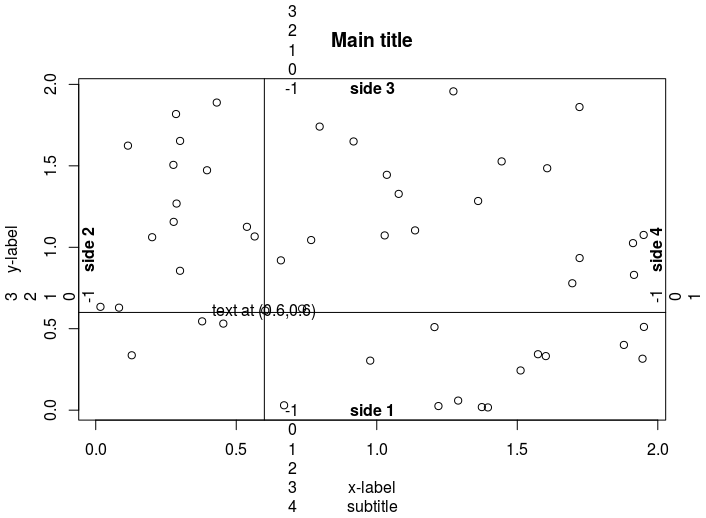
\includegraphics[width=\linewidth]{fig-5.png}
  \caption{La disposición de una gráfica estándar.}
  \label{fig:fig-5}
\end{figure}

Sin embargo, el hecho de que no se trace ningún gráfico no significa que no haya
pasado nada. El comando configura la región de trazado y los sistemas de
coordenadas como si realmente lo hubiera hecho. Para agregar los elementos de la
gráfica, evalúe lo siguiente:

\begin{lstlisting}[language=R]
> points(x,y)
> axis(1)
> axis(2,at=seq(0.2,1.8,0.2))
> box()
> title(main="Main title", sub="subtitle",xlab="x-label", ylab="y-label")
\end{lstlisting}

Observe cómo la llamada a \textt{axis} especifica un conjunto alternativo de
marcas de verificación (y etiquetas). Esta es una técnica común utilizada para
crear ejes especiales en un gráfico y también se puede utilizar para crear ejes
no equidistantes, así como ejes con etiquetado no numérico.

Trazar con \texttt{type="n"} es a veces una técnica útil porque tiene el efecto
secundario de dimensionar el área de la gráfica. Por ejemplo, para crear un
gráfico con diferentes colores para diferentes grupos, primero puede trazar
todos los datos con \texttt{type="n"}, asegurándose de que la región del gráfico
es lo suficientemente grande, y luego sumar los puntos para cada grupo usando
\texttt{points}. (Pasar un argumento vectorial para \texttt{col} es más
conveniente en este caso en particular.

%%%%%%%%%%%%%%%%%%%%%%%%%%%%%%%%%%%%%%%%%%%%%%%%%%%%%%%%%%%%%%%%%%%%%%%%%%%%%%%
\subsection{Utilizando \texttt{par}}
%%%%%%%%%%%%%%%%%%%%%%%%%%%%%%%%%%%%%%%%%%%%%%%%%%%%%%%%%%%%%%%%%%%%%%%%%%%%%%%

La función \texttt{par} permite un control increíblemente fino sobre los
detalles de un gráfico, aunque puede ser bastante confusa para los principiantes
(e incluso para los usuarios expertos a veces). La mejor estrategia puede ser
simplemente tratar de aprender algunos trucos útiles a la vez y de vez en cuando
tratar de resolver un problema en particular examinando la página de ayuda.

Algunos de los parámetros, pero no todos, también se pueden establecer mediante
parámetros a las funciones de dibujo, que también tienen algunos parámetros que
no se pueden establecer mediante \texttt{par}.  Cuando un parámetro se puede
establecer por ambos métodos, la diferencia es, generalmente que si algo se se
configuró mediante \texttt{par}, entonces permanecerá configurado
posteriormente.

La configuración de \texttt{par} permite controlar el ancho y el tipo de línea,
así como el tamaño de los caracteres y fuente de la letra, color, estilo de
cálculo de los ejes, tamaño de la gráfica y figuras, recortes, etc. Es posible
dividir una figura en varias subfiguras utilizando los parámetros \texttt{mfrow}
y \texttt{mfcol}.

Por ejemplo, los tamaños de margen predeterminados son algo más de 5, 4, 4 y 2
líneas.  Puede definir \texttt{par(mar=c(4,4,2,2)+0.1)} antes de graficar. Esto
quita una línea fuera del margen inferior y dos líneas fuera del margen superior
del gráfico, lo que reducirá la cantidad de espacios en blanco no utilizados
cuando no haya un título o subtítulo principal. Si se mira cuidadosamente, se
notará que la Figura \ref{fig:fig-5} tiene una región de trazado algo más
pequeña que las otras gráficas de este libro. Esto se debe a que las otras
gráficas se han realizado con márgenes reducidos por razones de composición
tipográfica.

Sin embargo, no tiene sentido describir los parámetros gráficos de forma
completa en este punto. En su lugar, volveremos a ellos, ya que los utilizaremos 
para gráficos específicos.

%%%%%%%%%%%%%%%%%%%%%%%%%%%%%%%%%%%%%%%%%%%%%%%%%%%%%%%%%%%%%%%%%%%%%%%%%%%%%%%
\subsection{Combining plots}
%%%%%%%%%%%%%%%%%%%%%%%%%%%%%%%%%%%%%%%%%%%%%%%%%%%%%%%%%%%%%%%%%%%%%%%%%%%%%%%
\newpage

\section{R programming}
\subsection{Flow control} \label{flowcontrol}
\subsection{Classes and generic functions}

\section{Data entry}
\subsection{Leyendo desde un archivo de texto} \label{readtextfile}
\subsection{Further details on read.table}
\subsection{The data editor}
\subsection{Interfacing to other programs}
\section{Ejercicios}

%%%%%%%%%%%%%%%%%%%%%%%%%%%%%%%%%%%%%%%%%%%%%%%%%%%%%%%%%%%%%%%%%%%%%%%%%%%%%%%
\chapter{Probabilidad y distribuciones}
%%%%%%%%%%%%%%%%%%%%%%%%%%%%%%%%%%%%%%%%%%%%%%%%%%%%%%%%%%%%%%%%%%%%%%%%%%%%%%%

Los conceptos de aleatoriedad y probabilidad son fundamentales para las
estadísticas. Es un hecho empírico que la mayoría de los experimentos e
investigaciones no son perfectamente reproducibles. El grado de
irreproducibilidad puede variar: Algunos experimentos en física pueden producir
datos que son exactos hasta muchos decimales, mientras que los datos sobre
sistemas biológicos son típicamente mucho menos confiables. Sin embargo, la
visión de los datos como algo que proviene de una distribución estadística es
vital para entender los métodos estadísticos. En esta sección se esbozan las
ideas básicas de probabilidad y las funciones que tiene \textbf{R} para el
muestreo aleatorio y el manejo de las distribuciones teóricas.

%%%%%%%%%%%%%%%%%%%%%%%%%%%%%%%%%%%%%%%%%%%%%%%%%%%%%%%%%%%%%%%%%%%%%%%%%%%%%%%
\section{Muestreo aleatorio}
%%%%%%%%%%%%%%%%%%%%%%%%%%%%%%%%%%%%%%%%%%%%%%%%%%%%%%%%%%%%%%%%%%%%%%%%%%%%%%%

Gran parte de los primeros trabajos en la teoría de la probabilidad se referían
a juegos y apuestas, basados en consideraciones de simetría. Por lo tanto, la
noción básica de una  muestra aleatoria es la de repartir de una baraja bien
barajada o recoger bolas numeradas de una urna bien revuelta.

En \textbf{R}, se pueden simular estas situaciones con la función
\texttt{sample}. Si quieres elegir cinco números al azar del conjunto de
\texttt{1:40}, entonces se puede escribir:

\begin{lstlisting}[language=R]
> sample(1:40,5)
[1] 36 37 26 24  3
\end{lstlisting}

El primer parámetro (\texttt{x}) es el vector de valores posibles de dónde
obtendremos la muestra y el segundo (\texttt{size}) es el tamaño de la muestra.
En realidad, \texttt{sampe(40,5)} sería suficiente ya que un solo número se
interpreta como la longitud de una secuencia de números enteros desde el 1.

Note que el comportamiento predeterminado de \texttt{sample} es el de
\textit{muestreo sin reemplazo}. Es decir, las muestras no contendrán ningún
número repetido, y \texttt{size} obviamente no puede ser mayor que la longitud
del vector a muestrear. Si quiere muestreo con reemplazo, entonces necesita
agregar el parámetro \texttt{replace=TRUE}.

El muestreo con reemplazo es adecuado para modelar lanzamientos de monedas o
lanzamientos de un dado. Así, por ejemplo, para simular 10 lanzamientos de
monedas podríamos escribir:

\begin{lstlisting}[language=R]
> sample(c("H","T"), 10, replace=T)
[1] "T" "T" "T" "T" "T" "H" "H" "T" "H" "T"
\end{lstlisting}

En un lanzamiento normal de monedas, la probabilidad de cara debe ser igual a la
probabilidad de cruz, pero la idea de un evento aleatorio no se limita a casos
simétricos.  Podría aplicarse igualmente bien a otros casos, como el resultado
exitoso de un procedimiento quirúrgico. Esperemos que haya más de un 50% de
posibilidades de que esto suceda. Puede simular datos con probabilidades no
simétricas para los resultados (por ejemplo, un 90\% de probabilidad de éxito)
usando el parámetro \texttt{prob} de \texttt{sample}, como ser:

\begin{lstlisting}[language=R]
> sample(c("succ", "fail"), 10, replace=T, prob=c(0.9, 0.1))
[1] "succ" "succ" "succ" "succ" "succ" "succ" "succ" "succ"
[9] "succ" "succ"
\end{lstlisting}

Sin embargo, esta puede no ser la mejor manera de generar una muestra de este
tipo. Ver la discusión posterior de la distribución binomial.

%%%%%%%%%%%%%%%%%%%%%%%%%%%%%%%%%%%%%%%%%%%%%%%%%%%%%%%%%%%%%%%%%%%%%%%%%%%%%%%
\section{Cálculos de probabilidad y combinatoria}
%%%%%%%%%%%%%%%%%%%%%%%%%%%%%%%%%%%%%%%%%%%%%%%%%%%%%%%%%%%%%%%%%%%%%%%%%%%%%%%

Volvamos al caso del muestreo sin reemplazo, específicamente
\texttt{sample(1:40,5)}. La probabilidad de obtener un número dado como ser, el
primero de la muestra debe ser de $1/40$, la del siguiente es de $1/39$, y así
sucesivamente. La probabilidad entonces  de obtener una determinada combinación
de 5 números,  debe ser de $1/(40 \times 39 \times 38 \times 37 \times 36)$.  En
\textbf{R}, puede utilizar la función \texttt{prod}, para calcular el producto
de un vector de números:

\begin{lstlisting}[language=R]
> 1/prod(40:36)
[1] 1.266449e-08
\end{lstlisting}

Sin embargo, tenga en cuenta que esta es la probabilidad de que se den los
números en un orden determinado. Si se tratara de un juego como el de la
lotería, entonces preferiría estar interesado en la probabilidad de adivinar
correctamente un determinado conjunto de cinco números.  Por lo tanto, también
es necesario incluir los casos que dan los mismos números pero en un orden
diferente.  Puesto que obviamente la probabilidad de cada caso va a ser la
misma, todo lo que tenemos que hacer es averiguar cuántos casos de este tipo hay
y multiplicarlos por eso. Hay cinco posibilidades para el primer número, y para
cada uno de ellos hay cuatro posibilidades para el segundo, y así sucesivamente;
es decir, el número es $5 \times 4 \times 3 \times 2 \times 1$. ¡Este número
también se escribe como $5!$ (factorial de 5)!. Así que la probabilidad de un
cupón ganador de la lotería, sería:

\begin{lstlisting}[language=R]
> prod(5:1)/prod(40:36)
[1] 1.519738e-06
\end{lstlisting}

Hay otra forma de llegar al mismo resultado. Note que como el conjunto real de
números es irrelevante, todos los conjuntos de cinco números deben tener la
misma probabilidad. Así que todo lo que tenemos que hacer es calcular el número
de maneras de elegir 5 números de un total de 40. Esto se puede definir como:

\begin{gather*}
\left(
    \begin{array}{c}
      40\\
      5
  \end{array}
\right) = \frac{40!}{5!35!} = 658008
\end{gather*} 

En \textbf{R}, se puede utilizar la función \texttt{choose} para calcular este
número, y por lo tanto la probabilidad es:

\begin{lstlisting}[language=R]
> 1/choose(40,5)
[1] 1.519738e-06
\end{lstlisting}

%%%%%%%%%%%%%%%%%%%%%%%%%%%%%%%%%%%%%%%%%%%%%%%%%%%%%%%%%%%%%%%%%%%%%%%%%%%%%%%
\section{Distribuciones discretas}
%%%%%%%%%%%%%%%%%%%%%%%%%%%%%%%%%%%%%%%%%%%%%%%%%%%%%%%%%%%%%%%%%%%%%%%%%%%%%%%

Al examinar las réplicas independientes de un experimento binario, normalmente
no nos interesaría saber si cada caso es un éxito o un fracaso, sino más bien el
número total de éxitos (o fracasos). Obviamente, este número es aleatorio ya que
depende de la salida aleatoria individual, y por lo tanto se le llama variable
aleatoria. En este caso, es una \textit{variable aleatoria} de valor discreto
que puede tomar valores 0, 1, .... \textit{n}, donde \textit{n} es el número de
réplicas. Las variables aleatorias continuas se verán más tarde.

A random variable X has a probability distribution that can be described using
point probabilities f ( x ) = P ( X = x ) or the cumulative distribution
function F ( x ) = P ( X <= x ) . In the case at hand, the distribution can be
worked out as having the point probabilities


\section{Continuous distributions}
\section{The built-in distributions in R}
\subsection{Densities}
\subsection{Cumulative distribution functions}
\subsection{Quantiles}
\subsection{Random numbers}
\section{Ejercicios}
\newpage



%%%%%%%%%%%%%%%%%%%%%%%%%%%%%%%%%%%%%%%%%%%%%%%%%%%%%%%%%%%%%%%%%%%%%%%%%%%%%%%
\chapter{Descriptive statistics and graphics}
%%%%%%%%%%%%%%%%%%%%%%%%%%%%%%%%%%%%%%%%%%%%%%%%%%%%%%%%%%%%%%%%%%%%%%%%%%%%%%%
\section{Resumen estadístico para un solo grupo} \label{resestad}
\section{Graphical display of distributions}
\section{Graphics for grouped data}
\section{Tables} \label{tables}
\section{Graphical display of tables}


%%%%%%%%%%%%%%%%%%%%%%%%%%%%%%%%%%%%%%%%%%%%%%%%%%%%%%%%%%%%%%%%%%%%%%%%%%%%%%%
\chapter{Manejo avanzado de datos}
%%%%%%%%%%%%%%%%%%%%%%%%%%%%%%%%%%%%%%%%%%%%%%%%%%%%%%%%%%%%%%%%%%%%%%%%%%%%%%%
\section{Recoding variables}
\subsection{The cut function}
\subsection{Manipulating factor levels}
\subsection{Working with dates}
\subsection{Recoding multiple variables}
\section{Conditional calculations}
\section{Combining and restructuring data frames}
\subsection{Appending frames} \label{appending frames}
\subsection{Merging data frames}
\subsection{Reshaping data frames}
\section{Per-group and per-case procedures}
\section{Time splitting}
\section{Ejercicios}



\end{document}
